%%%%%%%%%%%%%%%%%%%%%%%%%%%%%%%%%%%%%%%%%
% Masters/Doctoral Thesis 
% LaTeX Template
% Version 2.2 (21/11/15)
%
% This template has been downloaded from:
% http://www.LaTeXTemplates.com
%
% Version 2.x major modifications by:
% Vel (vel@latextemplates.com)
%
% This template is based on a template by:
% Steve Gunn (http://users.ecs.soton.ac.uk/srg/softwaretools/document/templates/)
% Sunil Patel (http://www.sunilpatel.co.uk/thesis-template/)
%
% Template license:
% CC BY-NC-SA 3.0 (http://creativecommons.org/licenses/by-nc-sa/3.0/)
%
%%%%%%%%%%%%%%%%%%%%%%%%%%%%%%%%%%%%%%%%%

%----------------------------------------------------------------------------------------
%	PACKAGES AND OTHER DOCUMENT CONFIGURATIONS
%----------------------------------------------------------------------------------------

\documentclass[
11pt, % The default document font size, options: 10pt, 11pt, 12pt
% oneside, % Two side (alternating margins) for binding by default, uncomment to switch to one side
english, % ngerman for German
singlespacing, % Single line spacing, alternatives: onehalfspacing or doublespacing
%draft, % Uncomment to enable draft mode (no pictures, no links, overfull hboxes indicated)
%nolistspacing, % If the document is onehalfspacing or doublespacing, uncomment this to set spacing in lists to single
%liststotoc, % Uncomment to add the list of figures/tables/etc to the table of contents
%toctotoc, % Uncomment to add the main table of contents to the table of contents
%parskip, % Uncomment to add space between paragraphs
% nohyperref, % Uncomment to not load the hyperref package
headsepline, % Uncomment to get a line under the header
]{MastersDoctoralThesis} % The class file specifying the document structure

\usepackage{caption}
\usepackage{subcaption}
\usepackage[utf8]{inputenc} % Required for inputting international characters
\usepackage[T1]{fontenc} % Output font encoding for international characters
\usepackage{xcolor}
\usepackage{palatino} % Use the Palatino font by default
\usepackage{listings}
\usepackage[backend=biber,style=numeric,natbib=true]{biblatex} % User the bibtex backend with the authoryear citation style (which resembles APA)
\usepackage[]{amsmath}
\addbibresource{Research.bib} % The filename of the bibliography

\usepackage[autostyle=true]{csquotes} % Required to generate language-dependent quotes in the bibliography
%----------------------------------------------------------------------------------------
%	MARGIN SETTINGS
%----------------------------------------------------------------------------------------

\geometry{
	paper=a4paper, % Change to letterpaper for US letter
	inner=2.5cm, % Inner margin
	outer=3.8cm, % Outer margin
	bindingoffset=2cm, % Binding offset
	top=1.5cm, % Top margin
	bottom=1.5cm, % Bottom margin
	%showframe,% show how the type block is set on the page
}

%----------------------------------------------------------------------------------------
%	THESIS INFORMATION
%----------------------------------------------------------------------------------------

\thesistitle{USPTO Patent Network: A statistical exploration of structural differences between examiner and applicant citations} % Your thesis title, this is used in the title and abstract, print it elsewhere with \ttitle
\supervisor{Dr. Markus \textsc{Brede}} % Your supervisor's name, this is used in the title page, print it elsewhere with \supname
\examiner{} % Your examiner's name, this is not currently used anywhere in the template, print it elsewhere with \examname
\degree{Data Science MSc} % Your degree name, this is used in the title page and abstract, print it elsewhere with \degreename
\author{Alun \textsc{Meredith}} % Your name, this is used in the title page and abstract, print it elsewhere with \authorname
\addresses{} % Your address, this is not currently used anywhere in the template, print it elsewhere with \addressname

\subject{Data Science} % Your subject area, this is not currently used anywhere in the template, print it elsewhere with \subjectname
\keywords{} % Keywords for your thesis, this is not currently used anywhere in the template, print it elsewhere with \keywordnames
\university{\href{http://www.southampton.ac.uk/}{University of Southampton}} % Your university's name and URL, this is used in the title page and abstract, print it elsewhere with \univname
\department{\href{http://www.ecs.soton.ac.uk/}{Electronics and Computer Science}} % Your department's name and URL, this is used in the title page and abstract, print it elsewhere with \deptname
\group{\href{http://www.aic.ecs.soton.ac.uk/}{Agents, Interaction and Complexity}} % Your research group's name and URL, this is used in the title page, print it elsewhere with \groupname
\faculty{\href{http://www.fpse.soton.ac.uk/}{Faculty of Physical Science and Engineering}} % Your faculty's name and URL, this is used in the title page and abstract, print it elsewhere with \facname

\hypersetup{pdftitle=\ttitle} % Set the PDF's title to your title
\hypersetup{pdfauthor=\authorname} % Set the PDF's author to your name
\hypersetup{pdfkeywords=\keywordnames} % Set the PDF's keywords to your keywords

\begin{document}

\frontmatter % Use roman page numbering style (i, ii, iii, iv...) for the pre-content pages

\pagestyle{plain} % Default to the plain heading style until the thesis style is called for the body content

%----------------------------------------------------------------------------------------
%	TITLE PAGE
%----------------------------------------------------------------------------------------

\begin{titlepage}
\begin{center}

\textsc{\LARGE \univname}\\[1.5cm] % University name
\textsc{\Large Masters Thesis}\\[0.5cm] % Thesis type

\HRule \\[0.4cm] % Horizontal line
{\huge \bfseries \ttitle}\\[0.4cm] % Thesis title
\HRule \\[1.5cm] % Horizontal line
 
\begin{minipage}{0.4\textwidth}
\begin{flushleft} \large
\emph{Author:}\\
{\authorname} % Author name - remove the \href bracket to remove the link
\end{flushleft}
\end{minipage}
\begin{minipage}{0.4\textwidth}
\begin{flushright} \large
\emph{Supervisor:} \\
{\supname} % Supervisor name - remove the \href bracket to remove the link  
\end{flushright}
\end{minipage}\\[3cm]
 
\large \textit{A thesis submitted in fulfillment of the requirements\\ for the degree of \degreename}\\[0.3cm] % University requirement text
\textit{in the}\\[0.4cm]
\groupname\\\deptname\\[2cm] % Research group name and department name
 
{\large \today}\\[4cm] % Date

\includegraphics[width = 0.3\linewidth]{Figures/southamptonLogo} % University/department logo - uncomment to place it

\pagebreak
\end{center}
\end{titlepage}

%----------------------------------------------------------------------------------------
%	TITLE PAGE (again)
%----------------------------------------------------------------------------------------

\begin{titlepage}
\begin{center}

\textsc{\LARGE \univname}\\[1.5cm] % University name
\textsc{\Large Masters Thesis}\\[0.5cm] % Thesis type

\HRule \\[0.4cm] % Horizontal line
{\huge \bfseries \ttitle}\\[0.4cm] % Thesis title
\HRule \\[1.5cm] % Horizontal line
 
\begin{minipage}{0.4\textwidth}
\begin{flushleft} \large
\emph{Author:}\\
{\authorname} % Author name - remove the \href bracket to remove the link
\end{flushleft}
\end{minipage}
\begin{minipage}{0.4\textwidth}
\begin{flushright} \large
\emph{Supervisor:} \\
{\supname} % Supervisor name - remove the \href bracket to remove the link  
\end{flushright}
\end{minipage}\\[3cm]
 
\large \textit{A thesis submitted in fulfilment of the requirements\\ for the degree of \degreename}\\[0.3cm] % University requirement text
\textit{in the}\\[0.4cm]
\groupname\\\deptname\\[2cm] % Research group name and department name
 
{\large \today}\\[4cm] % Date

\includegraphics[width = 0.3\linewidth]{Figures/southamptonLogo} % University/department logo - uncomment to place it
 
%\vfill
\end{center}
\end{titlepage}

%---------------------------------------------------------------------------------------
%	ABSTRACT PAGE
%----------------------------------------------------------------------------------------

\begin{abstract}
\addchaptertocentry{\abstractname} % Add the abstract to the table of contents

Patent citation networks describe the organisation and evolution of innovation. Here we conduct a statistical analysis of the structure of the USPTO citation network. We show that the network is currently log-normally distributed but that there has been an evolution to this state. We also separate citations based on the role of the individual citing it and show structural differences in how Examiners and Applicants make their citations and how disparate these two sub-networks are. We present evidence that the networks have evolved over time shifting to one dominated by the applicant citations.

\end{abstract}

%----------------------------------------------------------------------------------------
%	ACKNOWLEDGEMENTS
%----------------------------------------------------------------------------------------

\begin{acknowledgements}
\addchaptertocentry{\acknowledgementname} % Add the acknowledgements to the table of contents

Thanks to my supervisor Markus for all his mentor-ship over the last 3 months and everyone involved in the Data Science MSc for putting together a fantastic and inspirational course, as well as those studying with me, without whom I wouldn't have learnt nearly as much.

\end{acknowledgements}

%----------------------------------------------------------------------------------------
%	LIST OF CONTENTS/FIGURES/TABLES PAGES
%----------------------------------------------------------------------------------------

\tableofcontents % Prints the main table of contents

\listoffigures % Prints the list of figures

\listoftables % Prints the list of tables

%----------------------------------------------------------------------------------------
%	ABBREVIATIONS
%----------------------------------------------------------------------------------------

\begin{abbreviations}{ll} % Include a list of abbreviations (a table of two columns)

\textbf{USPTO} & \textbf{U}nited \textbf{S}tates \textbf{P}atent \textbf{O}ffice\\
\textbf{XML} & e\textbf{X}tensible \textbf{M}arkup \textbf{L}anguage\\
\textbf{SGML} & \textbf{S}tandard \textbf{G}eneralised \textbf{M}arkup \textbf{L}anguage\\
\textbf{ICE} &  \textbf{I}nternational \textbf{C}ommon \textbf{E}lement\\

\end{abbreviations}

%----------------------------------------------------------------------------------------
%	THESIS CONTENT - CHAPTERS
%----------------------------------------------------------------------------------------

\mainmatter % Begin numeric (1,2,3...) page numbering

\pagestyle{thesis} % Return the page headers back to the "thesis" style

% Include the chapters of the thesis as separate files from the Chapters folder
% Uncomment the lines as you write the chapters

%% Chapter 1

\chapter{Chapter Title Here} % Main chapter title

\label{Chapter1} % For referencing the chapter elsewhere, use \ref{Chapter1} 

%----------------------------------------------------------------------------------------

% Define some commands to keep the formatting separated from the content 
\newcommand{\keyword}[1]{\textbf{#1}}
\newcommand{\tabhead}[1]{\textbf{#1}}
\newcommand{\code}[1]{\texttt{#1}}
\newcommand{\file}[1]{\texttt{\bfseries#1}}
\newcommand{\option}[1]{\texttt{\itshape#1}}

%----------------------------------------------------------------------------------------

\section{Welcome and Thank You}
Welcome to this \LaTeX{} Thesis Template, a beautiful and easy to use template for writing a thesis using the \LaTeX{} typesetting system.

If you are writing a thesis (or will be in the future) and its subject is technical or mathematical (though it doesn't have to be), then creating it in \LaTeX{} is highly recommended as a way to make sure you can just get down to the essential writing without having to worry over formatting or wasting time arguing with your word processor.

\LaTeX{} is easily able to professionally typeset documents that run to hundreds or thousands of pages long. With simple mark-up commands, it automatically sets out the table of contents, margins, page headers and footers and keeps the formatting consistent and beautiful. One of its main strengths is the way it can easily typeset mathematics, even \emph{heavy} mathematics. Even if those equations are the most horribly twisted and most difficult mathematical problems that can only be solved on a super-computer, you can at least count on \LaTeX{} to make them look stunning.

%----------------------------------------------------------------------------------------

\section{Learning \LaTeX{}}

\LaTeX{} is not a \textsc{wysiwyg} (What You See is What You Get) program, unlike word processors such as Microsoft Word or Apple's Pages. Instead, a document written for \LaTeX{} is actually a simple, plain text file that contains \emph{no formatting}. You tell \LaTeX{} how you want the formatting in the finished document by writing in simple commands amongst the text, for example, if I want to use \emph{italic text for emphasis}, I write the \verb|\emph{text}| command and put the text I want in italics in between the curly braces. This means that \LaTeX{} is a \enquote{mark-up} language, very much like HTML.

\subsection{A (not so short) Introduction to \LaTeX{}}

If you are new to \LaTeX{}, there is a very good eBook -- freely available online as a PDF file -- called, \enquote{The Not So Short Introduction to \LaTeX{}}. The book's title is typically shortened to just \emph{lshort}. You can download the latest version (as it is occasionally updated) from here:
\url{http://www.ctan.org/tex-archive/info/lshort/english/lshort.pdf}

It is also available in several other languages. Find yours from the list on this page: \url{http://www.ctan.org/tex-archive/info/lshort/}

It is recommended to take a little time out to learn how to use \LaTeX{} by creating several, small `test' documents, or having a close look at several templates on:\\ 
\url{http://www.LaTeXTemplates.com}\\ 
Making the effort now means you're not stuck learning the system when what you \emph{really} need to be doing is writing your thesis.

\subsection{A Short Math Guide for \LaTeX{}}

If you are writing a technical or mathematical thesis, then you may want to read the document by the AMS (American Mathematical Society) called, \enquote{A Short Math Guide for \LaTeX{}}. It can be found online here:
\url{http://www.ams.org/tex/amslatex.html}
under the \enquote{Additional Documentation} section towards the bottom of the page.

\subsection{Common \LaTeX{} Math Symbols}
There are a multitude of mathematical symbols available for \LaTeX{} and it would take a great effort to learn the commands for them all. The most common ones you are likely to use are shown on this page:
\url{http://www.sunilpatel.co.uk/latex-type/latex-math-symbols/}

You can use this page as a reference or crib sheet, the symbols are rendered as large, high quality images so you can quickly find the \LaTeX{} command for the symbol you need.

\subsection{\LaTeX{} on a Mac}
 
The \LaTeX{} distribution is available for many systems including Windows, Linux and Mac OS X. The package for OS X is called MacTeX and it contains all the applications you need -- bundled together and pre-customized -- for a fully working \LaTeX{} environment and work flow.
 
MacTeX includes a custom dedicated \LaTeX{} editor called TeXShop for writing your `\file{.tex}' files and BibDesk: a program to manage your references and create your bibliography section just as easily as managing songs and creating playlists in iTunes.

%----------------------------------------------------------------------------------------

\section{Getting Started with this Template}

If you are familiar with \LaTeX{}, then you should explore the directory structure of the template and then proceed to place your own information into the \emph{THESIS INFORMATION} block of the \file{main.tex} file. You can then modify the rest of this file to your unique specifications based on your degree/university. Section \ref{FillingFile} on page \pageref{FillingFile} will help you do this. Make sure you also read section \ref{ThesisConventions} about thesis conventions to get the most out of this template.

If you are new to \LaTeX{} it is recommended that you carry on reading through the rest of the information in this document.

Before you begin using this template you should ensure that its style complies with the thesis style guidelines imposed by your institution. In most cases this template style and layout will be suitable. If it is not, it may only require a small change to bring the template in line with your institution's recommendations. These modifications will need to be done on the \file{MastersDoctoralThesis.cls} file.

\subsection{About this Template}

This \LaTeX{} Thesis Template is originally based and created around a \LaTeX{} style file created by Steve R.\ Gunn from the University of Southampton (UK), department of Electronics and Computer Science. You can find his original thesis style file at his site, here:
\url{http://www.ecs.soton.ac.uk/~srg/softwaretools/document/templates/}

Steve's \file{ecsthesis.cls} was then taken by Sunil Patel who modified it by creating a skeleton framework and folder structure to place the thesis files in. The resulting template can be found on Sunil's site here:
\url{http://www.sunilpatel.co.uk/thesis-template}

Sunil's template was made available through \url{http://www.LaTeXTemplates.com} where it was modified many times based on user requests and questions. Version 2.0 and onwards of this template represents a major modification to Sunil's template and is, in fact, hardly recognisable. The work to make version 2.0 possible was carried out by \href{mailto:vel@latextemplates.com}{Vel} and Johannes Böttcher.

%----------------------------------------------------------------------------------------

\section{What this Template Includes}

\subsection{Folders}

This template comes as a single zip file that expands out to several files and folders. The folder names are mostly self-explanatory:

\keyword{Appendices} -- this is the folder where you put the appendices. Each appendix should go into its own separate \file{.tex} file. An example and template are included in the directory.

\keyword{Chapters} -- this is the folder where you put the thesis chapters. A thesis usually has about six chapters, though there is no hard rule on this. Each chapter should go in its own separate \file{.tex} file and they can be split as:
\begin{itemize}
\item Chapter 1: Introduction to the thesis topic
\item Chapter 2: Background information and theory
\item Chapter 3: (Laboratory) experimental setup
\item Chapter 4: Details of experiment 1
\item Chapter 5: Details of experiment 2
\item Chapter 6: Discussion of the experimental results
\item Chapter 7: Conclusion and future directions
\end{itemize}
This chapter layout is specialised for the experimental sciences.

\keyword{Figures} -- this folder contains all figures for the thesis. These are the final images that will go into the thesis document.

\subsection{Files}

Included are also several files, most of them are plain text and you can see their contents in a text editor. After initial compilation, you will see that more auxiliary files are created by \LaTeX{} or BibTeX and which you don't need to delete or worry about:

\keyword{example.bib} -- this is an important file that contains all the bibliographic information and references that you will be citing in the thesis for use with BibTeX. You can write it manually, but there are reference manager programs available that will create and manage it for you. Bibliographies in \LaTeX{} are a large subject and you may need to read about BibTeX before starting with this. Many modern reference managers will allow you to export your references in BibTeX format which greatly eases the amount of work you have to do.

\keyword{MastersDoctoralThesis.cls} -- this is an important file. It is the class file that tells \LaTeX{} how to format the thesis. 

\keyword{main.pdf} -- this is your beautifully typeset thesis (in the PDF file format) created by \LaTeX{}. It is supplied in the PDF with the template and after you compile the template you should get an identical version.

\keyword{main.tex} -- this is an important file. This is the file that you tell \LaTeX{} to compile to produce your thesis as a PDF file. It contains the framework and constructs that tell \LaTeX{} how to layout the thesis. It is heavily commented so you can read exactly what each line of code does and why it is there. After you put your own information into the \emph{THESIS INFORMATION} block -- you have now started your thesis!

Files that are \emph{not} included, but are created by \LaTeX{} as auxiliary files include:

\keyword{main.aux} -- this is an auxiliary file generated by \LaTeX{}, if it is deleted \LaTeX{} simply regenerates it when you run the main \file{.tex} file.

\keyword{main.bbl} -- this is an auxiliary file generated by BibTeX, if it is deleted, BibTeX simply regenerates it when you run the \file{main.aux} file. Whereas the \file{.bib} file contains all the references you have, this \file{.bbl} file contains the references you have actually cited in the thesis and is used to build the bibliography section of the thesis.

\keyword{main.blg} -- this is an auxiliary file generated by BibTeX, if it is deleted BibTeX simply regenerates it when you run the main \file{.aux} file.

\keyword{main.lof} -- this is an auxiliary file generated by \LaTeX{}, if it is deleted \LaTeX{} simply regenerates it when you run the main \file{.tex} file. It tells \LaTeX{} how to build the \emph{List of Figures} section.

\keyword{main.log} -- this is an auxiliary file generated by \LaTeX{}, if it is deleted \LaTeX{} simply regenerates it when you run the main \file{.tex} file. It contains messages from \LaTeX{}, if you receive errors and warnings from \LaTeX{}, they will be in this \file{.log} file.

\keyword{main.lot} -- this is an auxiliary file generated by \LaTeX{}, if it is deleted \LaTeX{} simply regenerates it when you run the main \file{.tex} file. It tells \LaTeX{} how to build the \emph{List of Tables} section.

\keyword{main.out} -- this is an auxiliary file generated by \LaTeX{}, if it is deleted \LaTeX{} simply regenerates it when you run the main \file{.tex} file.

So from this long list, only the files with the \file{.bib}, \file{.cls} and \file{.tex} extensions are the most important ones. The other auxiliary files can be ignored or deleted as \LaTeX{} and BibTeX will regenerate them.

%----------------------------------------------------------------------------------------

\section{Filling in Your Information in the \file{main.tex} File}\label{FillingFile}

You will need to personalise the thesis template and make it your own by filling in your own information. This is done by editing the \file{main.tex} file in a text editor or your favourite LaTeX environment.

Open the file and scroll down to the second large block titled \emph{THESIS INFORMATION} where you can see the entries for \emph{University Name}, \emph{Department Name}, etc \ldots

Fill out the information about yourself, your group and institution. You can also insert web links, if you do, make sure you use the full URL, including the \code{http://} for this. If you don't want these to be linked, simply remove the \verb|\href{url}{name}| and only leave the name.

When you have done this, save the file and recompile \code{main.tex}. All the information you filled in should now be in the PDF, complete with web links. You can now begin your thesis proper!

%----------------------------------------------------------------------------------------

\section{The \code{main.tex} File Explained}

The \file{main.tex} file contains the structure of the thesis. There are plenty of written comments that explain what pages, sections and formatting the \LaTeX{} code is creating. Each major document element is divided into commented blocks with titles in all capitals to make it obvious what the following bit of code is doing. Initially there seems to be a lot of \LaTeX{} code, but this is all formatting, and it has all been taken care of so you don't have to do it.

Begin by checking that your information on the title page is correct. For the thesis declaration, your institution may insist on something different than the text given. If this is the case, just replace what you see with what is required in the \emph{DECLARATION PAGE} block.

Then comes a page which contains a funny quote. You can put your own, or quote your favourite scientist, author, person, and so on. Make sure to put the name of the person who you took the quote from.

Following this is the abstract page which summarises your work in a condensed way and can almost be used as a standalone document to describe what you have done. The text you write will cause the heading to move up so don't worry about running out of space.

Next come the acknowledgements. On this page, write about all the people who you wish to thank (not forgetting parents, partners and your advisor/supervisor).

The contents pages, list of figures and tables are all taken care of for you and do not need to be manually created or edited. The next set of pages are more likely to be optional and can be deleted since they are for a more technical thesis: insert a list of abbreviations you have used in the thesis, then a list of the physical constants and numbers you refer to and finally, a list of mathematical symbols used in any formulae. Making the effort to fill these tables means the reader has a one-stop place to refer to instead of searching the internet and references to try and find out what you meant by certain abbreviations or symbols.

The list of symbols is split into the Roman and Greek alphabets. Whereas the abbreviations and symbols ought to be listed in alphabetical order (and this is \emph{not} done automatically for you) the list of physical constants should be grouped into similar themes.

The next page contains a one line dedication. Who will you dedicate your thesis to?

Finally, there is the block where the chapters are included. Uncomment the lines (delete the \code{\%} character) as you write the chapters. Each chapter should be written in its own file and put into the \emph{Chapters} folder and named \file{Chapter1}, \file{Chapter2}, etc\ldots Similarly for the appendices, uncomment the lines as you need them. Each appendix should go into its own file and placed in the \emph{Appendices} folder.

After the preamble, chapters and appendices finally comes the bibliography. The bibliography style (called \option{authoryear}) is used for the bibliography and is a fully featured style that will even include links to where the referenced paper can be found online. Do not underestimate how grateful your reader will be to find that a reference to a paper is just a click away. Of course, this relies on you putting the URL information into the BibTeX file in the first place.

%----------------------------------------------------------------------------------------

\section{Thesis Features and Conventions}\label{ThesisConventions}

To get the best out of this template, there are a few conventions that you may want to follow.

One of the most important (and most difficult) things to keep track of in such a long document as a thesis is consistency. Using certain conventions and ways of doing things (such as using a Todo list) makes the job easier. Of course, all of these are optional and you can adopt your own method.

\subsection{Printing Format}

This thesis template is designed for double sided printing (i.e. content on the front and back of pages) as most theses are printed and bound this way. Switching to one sided printing is as simple as uncommenting the \option{oneside} option of the \code{documentclass} command at the top of the \file{main.tex} file. You may then wish to adjust the margins to suit specifications from your institution.

The headers for the pages contain the page number on the outer side (so it is easy to flick through to the page you want) and the chapter name on the inner side.

The text is set to 11 point by default with single line spacing, again, you can tune the text size and spacing should you want or need to using the options at the very start of \file{main.tex}. The spacing can be changed similarly by replacing the \option{singlespacing} with \option{onehalfspacing} or \option{doublespacing}.

\subsection{Using US Letter Paper}

The paper size used in the template is A4, which is the standard size in Europe. If you are using this thesis template elsewhere and particularly in the United States, then you may have to change the A4 paper size to the US Letter size. This can be done in the margins settings section in \file{main.tex}.

Due to the differences in the paper size, the resulting margins may be different to what you like or require (as it is common for institutions to dictate certain margin sizes). If this is the case, then the margin sizes can be tweaked by modifying the values in the same block as where you set the paper size. Now your document should be set up for US Letter paper size with suitable margins.

\subsection{References}

The \code{biblatex} package is used to format the bibliography and inserts references such as this one \parencite{Reference1}. The options used in the \file{main.tex} file mean that the in-text citations of references are formatted with the author(s) listed with the date of the publication. Multiple references are separated by semicolons (e.g. \parencite{Reference2, Reference1}) and references with more than three authors only show the first author with \emph{et al.} indicating there are more authors (e.g. \parencite{Reference3}). This is done automatically for you. To see how you use references, have a look at the \file{Chapter1.tex} source file. Many reference managers allow you to simply drag the reference into the document as you type.

Scientific references should come \emph{before} the punctuation mark if there is one (such as a comma or period). The same goes for footnotes\footnote{Such as this footnote, here down at the bottom of the page.}. You can change this but the most important thing is to keep the convention consistent throughout the thesis. Footnotes themselves should be full, descriptive sentences (beginning with a capital letter and ending with a full stop). The APA6 states: \enquote{Footnote numbers should be superscripted, [...], following any punctuation mark except a dash.} The Chicago manual of style states: \enquote{A note number should be placed at the end of a sentence or clause. The number follows any punctuation mark except the dash, which it precedes. It follows a closing parenthesis.}

The bibliography is typeset with references listed in alphabetical order by the first author's last name. This is similar to the APA referencing style. To see how \LaTeX{} typesets the bibliography, have a look at the very end of this document (or just click on the reference number links in in-text citations).

\subsubsection{A Note on bibtex}

The bibtex backend used in the template by default does not correctly handle unicode character encoding (i.e. "international" characters). You may see a warning about this in the compilation log and, if your references contain unicode characters, they may not show up correctly or at all. The solution to this is to use the biber backend instead of the outdated bibtex backend. This is done by finding this in \file{main.tex}: \option{backend=bibtex} and changing it to \option{backend=biber}. You will then need to delete all auxiliary BibTeX files and navigate to the template directory in your terminal (command prompt). Once there, simply type \code{biber main} and biber will compile your bibliography. You can then compile \file{main.tex} as normal and your bibliography will be updated. An alternative is to set up your LaTeX editor to compile with biber instead of bibtex, see \href{http://tex.stackexchange.com/questions/154751/biblatex-with-biber-configuring-my-editor-to-avoid-undefined-citations/}{here} for how to do this for various editors.

\subsection{Tables}

Tables are an important way of displaying your results, below is an example table which was generated with this code:

{\small
\begin{verbatim}
\begin{table}
\caption{The effects of treatments X and Y on the four groups studied.}
\label{tab:treatments}
\centering
\begin{tabular}{l l l}
\toprule
\tabhead{Groups} & \tabhead{Treatment X} & \tabhead{Treatment Y} \\
\midrule
1 & 0.2 & 0.8\\
2 & 0.17 & 0.7\\
3 & 0.24 & 0.75\\
4 & 0.68 & 0.3\\
\bottomrule\\
\end{tabular}
\end{table}
\end{verbatim}
}

\begin{table}
\caption{The effects of treatments X and Y on the four groups studied.}
\label{tab:treatments}
\centering
\begin{tabular}{l l l}
\toprule
\tabhead{Groups} & \tabhead{Treatment X} & \tabhead{Treatment Y} \\
\midrule
1 & 0.2 & 0.8\\
2 & 0.17 & 0.7\\
3 & 0.24 & 0.75\\
4 & 0.68 & 0.3\\
\bottomrule\\
\end{tabular}
\end{table}

You can reference tables with \verb|\ref{<label>}| where the label is defined within the table environment. See \file{Chapter1.tex} for an example of the label and citation (e.g. Table~\ref{tab:treatments}).

\subsection{Figures}

There will hopefully be many figures in your thesis (that should be placed in the \emph{Figures} folder). The way to insert figures into your thesis is to use a code template like this:
\begin{verbatim}
\begin{figure}
\centering
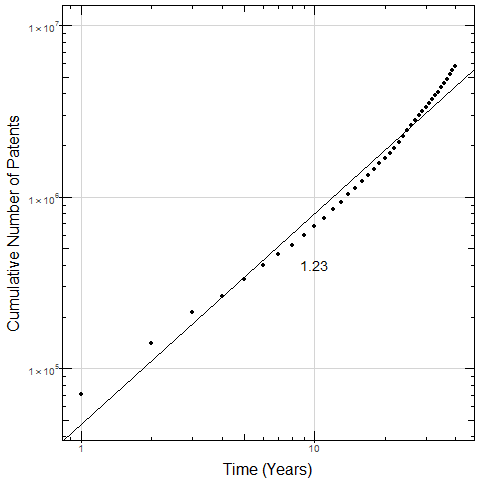
\includegraphics{Figures/CumulativePatents1}
\decoRule
\caption[An Electron]{An electron (artist's impression).}
\label{fig:Electron}
\end{figure}
\end{verbatim}
Also look in the source file. Putting this code into the source file produces the picture of the electron that you can see in the figure below.

\begin{figure}[h]
\centering
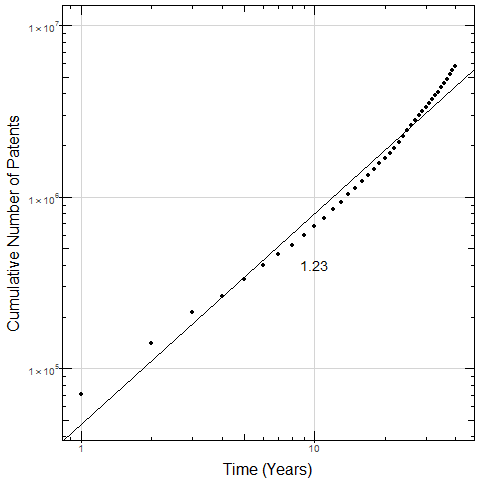
\includegraphics[width = 0.7\linewidth]{Figures/CumulativePatents1}
\decoRule
\caption[An Electron]{An electron (artist's impression).}
\label{fig:Electron}
\end{figure}

Sometimes figures don't always appear where you write them in the source. The placement depends on how much space there is on the page for the figure. Sometimes there is not enough room to fit a figure directly where it should go (in relation to the text) and so \LaTeX{} puts it at the top of the next page. Positioning figures is the job of \LaTeX{} and so you should only worry about making them look good!

Figures usually should have captions just in case you need to refer to them (such as in Figure~\ref{fig:Electron}). The \verb|\caption| command contains two parts, the first part, inside the square brackets is the title that will appear in the \emph{List of Figures}, and so should be short. The second part in the curly brackets should contain the longer and more descriptive caption text.

The \verb|\decoRule| command is optional and simply puts an aesthetic horizontal line below the image. If you do this for one image, do it for all of them.

\LaTeX{} is capable of using images in pdf, jpg and png format.

\subsection{Typesetting mathematics}

If your thesis is going to contain heavy mathematical content, be sure that \LaTeX{} will make it look beautiful, even though it won't be able to solve the equations for you.

The \enquote{Not So Short Introduction to \LaTeX} (available on \href{http://www.ctan.org/tex-archive/info/lshort/english/lshort.pdf}{CTAN}) should tell you everything you need to know for most cases of typesetting mathematics. If you need more information, a much more thorough mathematical guide is available from the AMS called, \enquote{A Short Math Guide to \LaTeX} and can be downloaded from:
\url{ftp://ftp.ams.org/pub/tex/doc/amsmath/short-math-guide.pdf}

There are many different \LaTeX{} symbols to remember, luckily you can find the most common symbols in \href{http://ctan.org/pkg/comprehensive}{The Comprehensive \LaTeX~Symbol List}.

You can write an equation, which is automatically given an equation number by \LaTeX{} like this:
\begin{verbatim}
\begin{equation}
E = mc^{2}
\label{eqn:Einstein}
\end{equation}
\end{verbatim}

This will produce Einstein's famous energy-matter equivalence equation:
\begin{equation}
E = mc^{2}
\label{eqn:Einstein}
\end{equation}

All equations you write (which are not in the middle of paragraph text) are automatically given equation numbers by \LaTeX{}. If you don't want a particular equation numbered, use the unnumbered form:
\begin{verbatim}
\[ a^{2}=4 \]
\end{verbatim}

%----------------------------------------------------------------------------------------

\section{Sectioning and Subsectioning}

You should break your thesis up into nice, bite-sized sections and subsections. \LaTeX{} automatically builds a table of Contents by looking at all the \verb|\chapter{}|, \verb|\section{}|  and \verb|\subsection{}| commands you write in the source.

The Table of Contents should only list the sections to three (3) levels. A \verb|chapter{}| is level zero (0). A \verb|\section{}| is level one (1) and so a \verb|\subsection{}| is level two (2). In your thesis it is likely that you will even use a \verb|subsubsection{}|, which is level three (3). The depth to which the Table of Contents is formatted is set within \file{MastersDoctoralThesis.cls}. If you need this changed, you can do it in \file{main.tex}.

%----------------------------------------------------------------------------------------

\section{In Closing}

You have reached the end of this mini-guide. You can now rename or overwrite this pdf file and begin writing your own \file{Chapter1.tex} and the rest of your thesis. The easy work of setting up the structure and framework has been taken care of for you. It's now your job to fill it out!

Good luck and have lots of fun!

\begin{flushright}
Guide written by ---\\
Sunil Patel: \href{http://www.sunilpatel.co.uk}{www.sunilpatel.co.uk}\\
Vel: \href{http://www.LaTeXTemplates.com}{LaTeXTemplates.com}
\end{flushright}

%%----------------------------------------------------------------------------------------
%	SECTION 1
%----------------------------------------------------------------------------------------


% Lorem ipsum dolor sit amet, consectetur adipiscing elit. Aliquam ultricies lacinia euismod. Nam tempus risus in dolor rhoncus in interdum enim tincidunt. Donec vel nunc neque. In condimentum ullamcorper quam non consequat. Fusce sagittis tempor feugiat. Fusce magna erat, molestie eu convallis ut, tempus sed arcu. Quisque molestie, ante a tincidunt ullamcorper, sapien enim dignissim lacus, in semper nibh erat lobortis purus. Integer dapibus ligula ac risus convallis pellentesque.

% \begin{figure}
% \centering
% \begin{subfigure}{.5\textwidth}
%   \centering
%   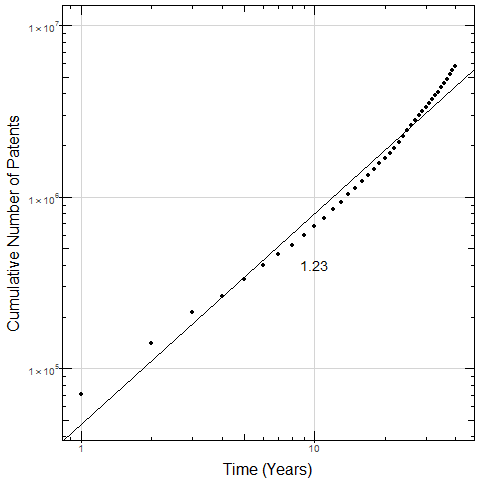
\includegraphics[width=0.7\linewidth]{Figures/CumulativePatents1}
%  \caption[CumPatents1]{\small Generalised linear model $y = x^\alpha $, fitted to all the data-points}
% \label{fig:CumPatents1}
% \end{subfigure}%
% \begin{subfigure}{.5\textwidth}
%   \centering
%   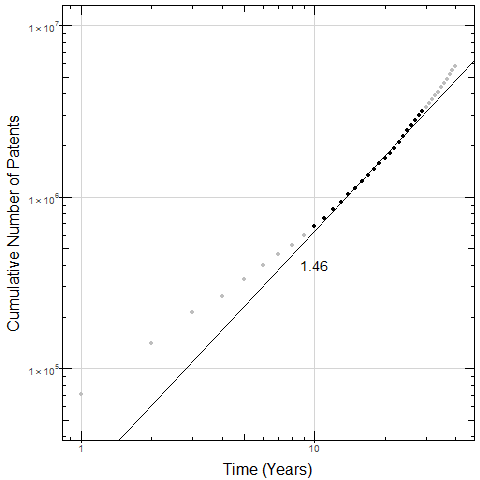
\includegraphics[width=0.7\linewidth]{Figures/CumulativePatents2}
%   \caption[CumPatents1]{\small Generalised linear model $y = x^\alpha $, fitted only to the years 1986 to 2005}
% \label{fig:CumPatents2}
% \end{subfigure}
% \caption[Power-law fit for cumulative number of patents granted each year]{The cumulative number of patents granted from 1976 to 2015, plotted on a log-log scales}
% \label{fig:CumPatents}
% \end{figure}

% %-----------------------------------
% %	SUBSECTION 1
% %-----------------------------------

% Nunc posuere quam at lectus tristique eu ultrices augue venenatis. Vestibulum ante ipsum primis in faucibus orci luctus et ultrices posuere cubilia Curae; Aliquam erat volutpat. Vivamus sodales tortor eget quam adipiscing in vulputate ante ullamcorper. Sed eros ante, lacinia et sollicitudin et, aliquam sit amet augue. In hac habitasse platea dictumst.

% \begin{figure}
% \centering
% \begin{subfigure}{.3\linewidth}
%   \centering
%   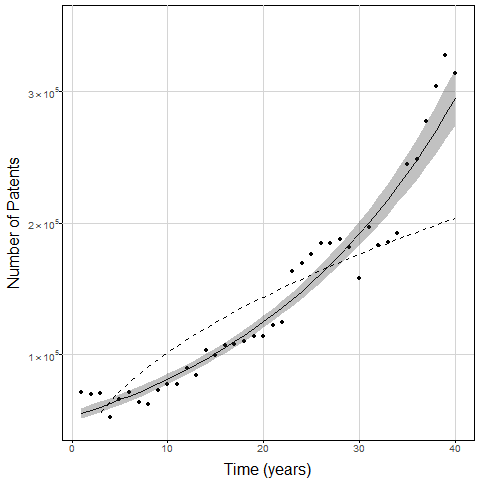
\includegraphics[width=0.9\linewidth]{Figures/patentCountFit}
%  \caption[CumPatents1]{\footnotesize Patents granted per year}
% \label{fig:patentCountFit}
% \end{subfigure}%
% \begin{subfigure}{.3\linewidth}
%   \centering
%   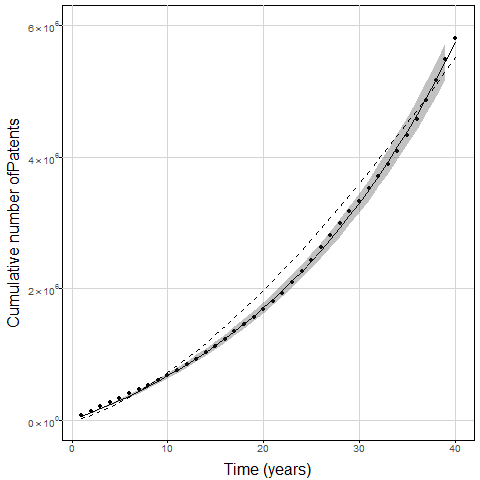
\includegraphics[width=0.9\linewidth]{Figures/patentCountFit_cum}
%   \caption[CumPatents1]{\footnotesize Cumulative number of patents granted}
% \label{fig:patentCountFit_cum}
% \end{subfigure}
% \begin{subfigure}{.3\linewidth}
%   \centering
%   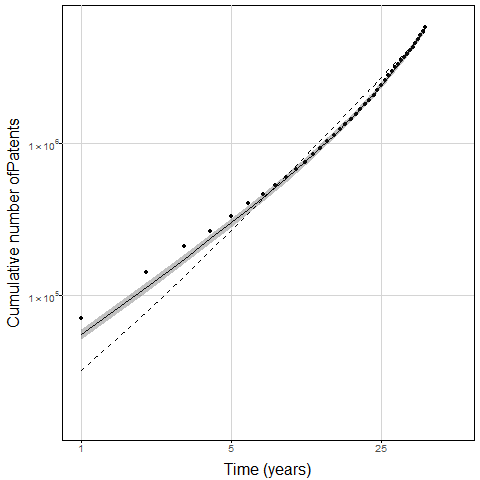
\includegraphics[width=0.9\linewidth]{Figures/patentCountFit_cum_loglog}
%   \caption[CumPatents1]{\footnotesize Cumulative patents granted on a log-log scale}
% \label{fig:patentCountFit_cum_loglog}
% \end{subfigure}
% \caption[Exponential fit for number of patents granted each year]{Power law and exponential fits for cumulative number of patents published each year}
% \label{fig:cumulativePatentFits}
% \end{figure}

%-----------------------------------
%	SUBSECTION 2
%-----------------------------------

% Morbi rutrum odio eget arcu adipiscing sodales. Aenean et purus a est pulvinar pellentesque. Cras in elit neque, quis varius elit. Phasellus fringilla, nibh eu tempus venenatis, dolor elit posuere quam, quis adipiscing urna leo nec orci. Sed nec nulla auctor odio aliquet consequat. Ut nec nulla in ante ullamcorper aliquam at sed dolor. Phasellus fermentum magna in augue gravida cursus. Cras sed pretium lorem. Pellentesque eget ornare odio. Proin accumsan, massa viverra cursus pharetra, ipsum nisi lobortis velit, a malesuada dolor lorem eu neque.


% \begin{figure}
% \centering
% \begin{subfigure}{.5\textwidth}
%   \centering
%   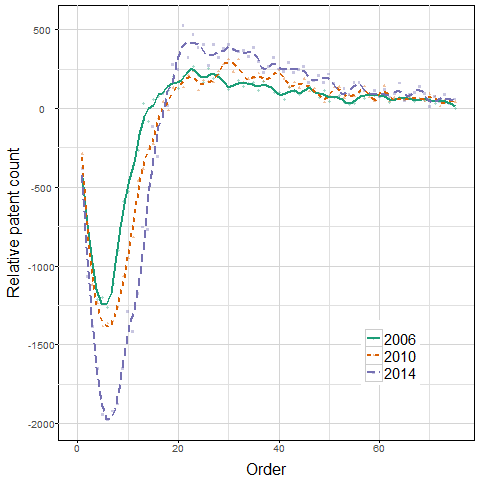
\includegraphics[width=0.7\linewidth]{Figures/parsingErrorsPerOrder}
%  \caption[CumPatents1]{\small Generalised linear model $y = x^\alpha $, fitted to all the data-points}
% \label{fig:parsingErrorsPerOrder}
% \end{subfigure}%
% \begin{subfigure}{.5\textwidth}
%   \centering
%   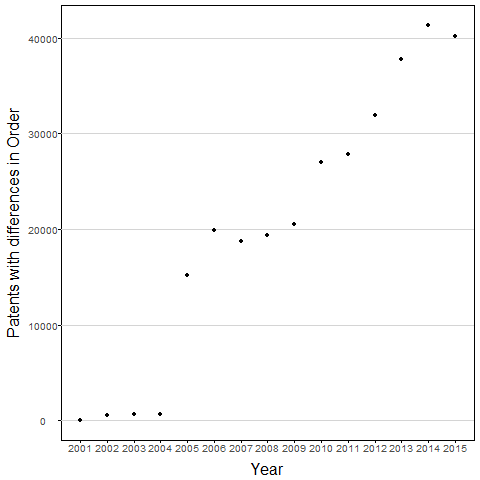
\includegraphics[width=0.7\linewidth]{Figures/parsingErrorsPerYear}
%   \caption[CumPatents1]{\small Generalised linear model $y = x^\alpha $, fitted only to the years 1986 to 2005}
% \label{fig:parsingErrorsPerYear}
% \end{subfigure}
% \caption[Differences in different parsing methods]{Number of patents with different values for order computed by (1) when parsing original data, (2) using a mapReduce on citations table.}
% \end{figure}

%----------------------------------------------------------------------------------------
%	SECTION 2
%----------------------------------------------------------------------------------------

% \section{Main Section 2}

% Sed ullamcorper quam eu nisl interdum at interdum enim egestas. Aliquam placerat justo sed lectus lobortis ut porta nisl porttitor. Vestibulum mi dolor, lacinia molestie gravida at, tempus vitae ligula. Donec eget quam sapien, in viverra eros. Donec pellentesque justo a massa fringilla non vestibulum metus vestibulum. Vestibulum in orci quis felis tempor lacinia. Vivamus ornare ultrices facilisis. Ut hendrerit volutpat vulputate. Morbi condimentum venenatis augue, id porta ipsum vulputate in. Curabitur luctus tempus justo. Vestibulum risus lectus, adipiscing nec condimentum quis, condimentum nec nisl. Aliquam dictum sagittis velit sed iaculis. Morbi tristique augue sit amet nulla pulvinar id facilisis ligula mollis. Nam elit libero, tincidunt ut aliquam at, molestie in quam. Aenean rhoncus vehicula hendrerit.

% \begin{figure}
% \centering
%  \centering
%  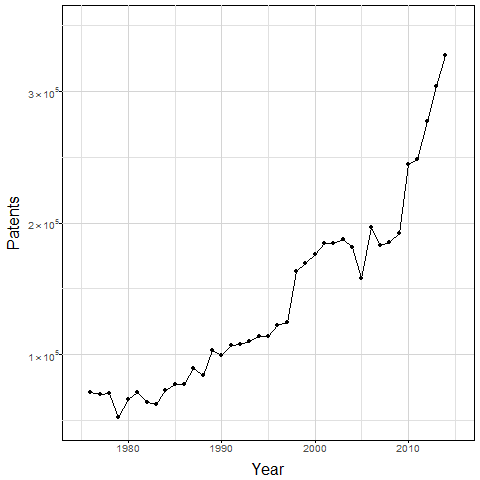
\includegraphics[width=0.7\linewidth]{Figures/PatentCountVsYear}
% \caption[Number of patents granted each year]{Number of patents granted each year from 1976 to 2015}
% \label{fig:PatentCountVsYear}
% \end{figure}

% \begin{figure}
% \centering
%   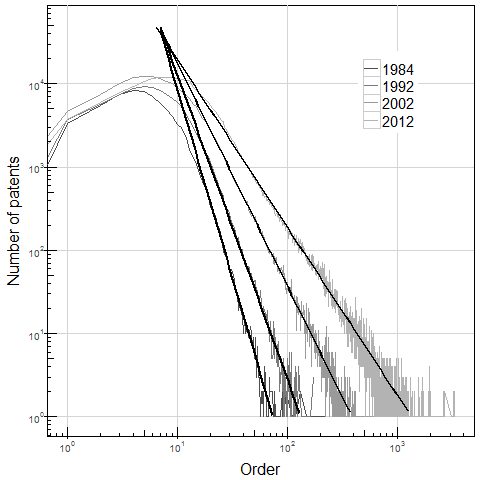
\includegraphics[width=0.7\linewidth]{Figures/OrderDistribution}
%   \caption[Degree Distribution]{Degree distribution (number of citations for each patent) on a log-log scale shown for years 1984,1992,2002,2012. Fit with generalized linear model of the form $y ~ x^\alpha$ yielding exponents of -...,-...,-... and -... respectively}
% \label{fig:OrderDistribution}
% \end{figure}

%----------------------------------------------------------------------------------------
%	SECTION 3
%----------------------------------------------------------------------------------------

% \section{Main Section 3}

% Sed ullamcorper quam eu nisl interdum at interdum enim egestas. Aliquam placerat justo sed lectus lobortis ut porta nisl porttitor. Vestibulum mi dolor, lacinia molestie gravida at, tempus vitae ligula. Donec eget quam sapien, in viverra eros. Donec pellentesque justo a massa fringilla non vestibulum metus vestibulum. Vestibulum in orci quis felis tempor lacinia. Vivamus ornare ultrices facilisis. Ut hendrerit volutpat vulputate. Morbi condimentum venenatis augue, id porta ipsum vulputate in. Curabitur luctus tempus justo. Vestibulum risus lectus, adipiscing nec condimentum quis, condimentum nec nisl. Aliquam dictum sagittis velit sed iaculis. Morbi tristique augue sit amet nulla pulvinar id facilisis ligula mollis. Nam elit libero, tincidunt ut aliquam at, molestie in quam. Aenean rhoncus vehicula hendrerit.

% \begin{figure}
% \centering
% \begin{subfigure}{.5\textwidth}
%   \centering
%   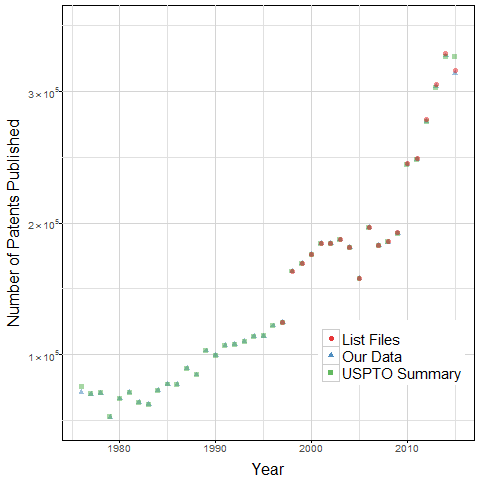
\includegraphics[width=0.7\linewidth]{Figures/patentsCompared}
%  \caption{Number of Patents parsed each year from each source}
% \label{fig:patentsCompared}
% \end{subfigure}%
% \begin{subfigure}{.5\textwidth}
%   \centering
%   
\includegraphics[width=0.7\linewidth]{Figures/patentsDiff}
%   \caption{\footnotesize Difference between number of Patents parsed from different sources and parsed data}
% \label{fig:patentsDiff}
% \end{subfigure}
% \caption[Difference between number of patents parsed from different sources]{\footnotesize The number of Patents granted each year according to 3 sources: Parsed data; a USPTO report and the .lst files.}
% \label{fig:patentCountsTest}
% \end{figure} 
% Chapter Template

\chapter{Introduction} % Main chapter title

\label{Chapter1} % Change X to a consecutive number; for referencing this chapter elsewhere, use \ref{ChapterX}

Patent networks are intrinsically linked to innovation and the economy. Although work has been done to extract economic meaning from these networks, economic growth through innovation is not well understood, and the value of a patent within these networks is often simplified to simply be the number of times they are cited.

Patents are a legal document claiming ownership of innovation. Through this process patent citations are legal obligations to reference 'prior art' any of which are initially missing from the application are added by the patent examiner. The objectivity of the examiner and legal basis for citations is what differentiates them from other bibliographic citation networks such as academic citations. 

Patents and by proxy innovation can be viewed as a combinatorial process \cite{youn2015invention}. In this way innovation like research 'stands on the shoulders of giants'. Through a greater understanding of the formation and evolution of the network insights can be gained into the process of innovation which impacts econometrics and companies trying to identify areas to direct their research alike. Many believe that over the last ten years we are in the middle of technological information revolution \cite{castells2011rise} and understanding the extent and impact of this on innovation. 

The US patent office database offers an opportunity for analysis as one of the largest patent collections openly available. Its large scale encompasses all the patents granted in the US from 1986 - 2015 in a structured although messy form, with more than 5 million patents and 110 million citations over the 30 year period.  The scale of the database and large number of features allows for unique insight into the structure of patent citation networks although along with the messiness requires big data solutions to achieve this. The USPTO network is relatively enclosed network with 84.5\% of its citations being internal since 2005 relative to a large scale study of academic citations which had 19-36 \% internal citations \cite{redner2004citation}. 

The aims of this project is to use the USPTO database in order to conduct some exploratory analysis and gain some statistical insight into the structure and evolution of the network and how it may be changing over the lifespan of the network, in particular the last 10 years. 

\section{Dissertation Structure}
This dissertation is organised as follows: In Chapter 2 there is a review of the literature and history of patent network research. In chapter 3 the data pipeline is explained, describing the processes by which the data has been parsed, cleaned and feature engineered before analysis could be done. Chapter 4 describes the analysis and discussion in a narrative flow, starting with some overviews of the network and reproduction of the work of Valverde et al. before analysing the coloured network of two classes of citation based on who contributed the citation to the patent. In chapter 5 the basic results are reviewed, implications and further work discussed. 

% Chapter Template

\chapter{Literature Review} % Main chapter title

\label{Chapter2} % Change X to a consecutive number; for referencing this chapter elsewhere, use \ref{ChapterX}

%----------------------------------------------------------------------------------------
%	Literature Review
%----------------------------------------------------------------------------------------
\section{History}

The study of information networks has seen a growing interest in the past 20 years as the networked systems become more and more popular and integral to modern society through revolutions in communication with email and mobile phones, revolutions in content consumption with the internet and revolutions in system architecture with the internet of things and agent based systems. 

Until recently many of these networks were treated as variations of random graphs, where edges (links) are attached to a set of vertices (nodes) sequentially through a random process \cite{erdds1959random,erd6s1960evolution}. However many networks have been shown to display characteristics not present in random graphs so different models with different attachment mechanisms are required. 

A 'Complex Network' is a macroscopic description of systems in which emergent macroscopic behaviour is produced from the small scale interactions, for example the climate is emergent from the interaction of different weather systems \cite{steinhaeuser2011complex}. These networks are loosely divided into two main classes: 'small world' and 'scale-free' networks. Small world networks are known for their short maximum path length between two nodes, producing characteristics like the 'Six Degrees of Separation'. These networks are highly clustered with long distance links between those clusters \cite{watts1998collective}. Scale-free networks however typically are not strongly clustered and are known for the distribution of edges across nodes (degree) following a power-law $f(x) \sim x^{-\alpha}$, this is sometimes also known by Zipf's law or a Pareto distribution \cite{zipf1935psycho}. This distribution has the property that there is no characteristic scale for the network. A typical scale means that each node has about the same consistent numbers of links producing structures similar to lattices so having no typical scale produces very unstructured networks. 

Scale-free networks are often characterised by a 'rich get richer' phenomenon, known as the Matthew effect \cite{merton1968matthew}. Both Price and Barabási present a 'preferential attachment' mechanism to model this effect where new edges are attached to nodes with probability as a linear function to the number of edges of that node to produce a power-law distribution \cite{albert2002statistical,price1976general}. 

\section{Bibliographic Networks}

Bibliographic networks are networks of authors and/or their works. Examples of these include collaboration networks, where links are formed from instances of author collaboration and citation networks where authors cite other works to be related. Academic citation and collaboration networks were some of the earliest identified as complex networks \cite{albert2002statistical}. 

The statistical nature of many complex networks, including patent networks is still being debated. This forms two fundamental questions: what is the functional form of the underlying distribution and what mechanisms form this distribution, these primarily try to identify power-law distributions and preferential attachment mechanisms although more recently research has extended preferential attachment with additional mechanisms such as ageing terms and fitness models. Answering the first question is difficult as log-normal curves can be very similar to power-law curves under the correct parameters. Clauset et al. describes a method for differentiating between these distributions using bootstrapping methods to discount unlikely distributions and log-likelihood ratios to compare two functional forms \cite{clauset2009power}. Although preferential attachment produces power-laws, a power-law is not sufficient to show presence of preferential attachment. Power-laws have been shown to be produced by other mechanisms such as a multiplication of many random processes \cite{newman2005power}. Log-normal distributions have also been shown to be produced by random multiplicative processes but also sub-linear preferential attachment \cite{redner2000random}. Therefore preferential attachment must be identified independently of the distributions functional form.  

In academic citation networks there has been recent research in the mechanics behind citations such as the propagation of errors which suggests 70 - 80\% of citations are copy and pasted from a secondary source \cite{simkin2005stochastic} or the study of redundant edges to show that the majority of references (~70\%) are secondary \cite{clough2015transitive}. Scientific citation networks have been shown to have characteristics consistent with a preferential attachment mechanism and Weibull ageing term \cite{borner2004simultaneous}.

Multi-dimensional networks are a generalisation of networks combining networks of nodes with multiple classes of link. The study of these networks has become one of the fastest growing areas of research in network science offering generalised diagnostics which can account for differences in nature between the links as well new insights \cite{hardtoSpell}.

\section{Patent Networks}

The main differentiating factor between academic citations and those found in patent networks is the stricter legal scope of citations in patents. Patents have a legal requirement to cite all 'prior art' from which the patent is based. This is a more narrow definition of a citation but also more exhaustive because if a 'prior art' is not cited in the application ideally a patent examiner will add it to the document. There is a larger body of research on academic citation networks due to the inherent domain knowledge researchers have with the field and because it was among the first to be identified as scale-free \cite{albert2002statistical}.

In 2007 Cs'ardi et al. published the first paper examining the US patent office database from a graph theoretical perspective \cite{csardi2007modeling}. They did this by by applying a basic model that assumes the attractiveness of a node (rate at which new nodes attach to it) is a function of the age and number of citations of the node. Normalising for the growth of the patent network over time they found the total attractiveness of the system over time could only be replicated with a super-linear preferential attachment model. They also explore the idea that an increase in the number of citations per patent over time has been coupled with a fundamental change in the structure of the network. Finding that the level of stratification starts to increase in alignment with the higher citation rates. 

Valverde et al. \cite{valverde2007topology} also analyses the data-set from a graph-theoretical perspective suggesting a form for the extended power law for the in-degree distribution, this functional form converges to a power law for high orders and an exponential for low orders. They also explore the clustering and modularity of the system. The clustering coefficient being approximately inversely proportional to the number of citations, suggesting a hierarchical structure. Finally they disagree with Cs'ardi et al. finding a linear preferential attachment. 

A recent study builds exposes the danger of relying on simple models studying the patent network as a whole \cite{gress2010properties}. Bernard Gress (2009) investigated the ratios between citations given and received in different technology groups. High number and diversity of citations given was treated as an indication of generality and number of citations received of productivity and originality. He then compared these measures and how they varied over time for different technology categories. He primarily concludes that these categories are fundamentally different therefore research needs to take this into account. 

Byungun Yoon \cite{yoon2004text} built a patent network from weighted term similarities of patent documents rather than bibliometric citations; using standard bag of words methods and comparing these measures to analogies in citation networks. Through inspection they argue that the centrality of their network yields a more relevant approximation of impact because it is less biased by age and preferential attachment mechanisms. 

As patents are a representation of innovation many studies try to measure the impact of a patent. Network based techniques often limit themselves to using the number of citations received as a measure of impact, however there is a lot of debate as to what extent this measure is valid and how these can be improved. 

\subsection{Innovation Networks}

There is a body of research exploring the analogy between the evolution of innovation and biological evolution. The premise is that each invention is built from the recombination of previous inventions. The two models have their differences, for example there is a limited concept of 'death' in innovation as very old patents may still be cited by new ones and it is hard to think of bibliometric patent networks as direct lineages. 

Yeoun et al. \cite{youn2015invention} explores this idea of invention as a recombination process by looking at the use of technology codes in patents as a proxy for novelty. Technology codes map the technological niche of a patent into categories and subcategories. Patents can have combinations of technology codes. They show that as the number of patents increases the number of new codes being generated falls off while new code combinations maintains a power-law, concluding new technologies has a minimal role relative to recombination. They also show that 40\% of patents use existing combinations vs. new ones suggesting these are incremental improvements. 

Technology code combination distributions do not age in the same way as bibliometric citations, codes appear not to age with 99\% of codes being used at least once every 7 years. 

They also look at the dissimilarity of the codes as a proxy for novelty. If a patent is used in a very different field from its parents it is argued that it is more likely to be a bigger leap in novelty. Categorising patents as either narrow or broad and using count as a metric, we only get a sense how novelty has changed with time and not any of the network factors which may be present here, such as the distribution of novelty could be a power law or the degree of novelty can be a measure of linkage between clusters. 

The limitations of the evolutionary analogy are loosely addressed warning that citations in patents aren't directly related to lineage but about carving a legal niche and there being no good metric of fitness for patents. 

Buchanan et al.\cite{buchanan2011measuring} glosses over some of these limitations, using the number of citations a patent has as an "impact" metric, a proxy for fitness. Prior art citations also function as a proxy for combinatorial lineage. They tell the story of the most cited patents in the network over the past 30 years and show that such a distribution of citations cannot come from random natural selection and therefore must be due to adaptive selection in an evolutionary model of innovation. This argument is an evolutionary perspective on the random network vs. preferential attachment network differentiation. 

They focus on showing this idea more robustly incorporating a multitude of normalisation techniques and simulating a null hypothesis random network model by sampling existing data, rather than building a clean model from scratch. Observing the familiar hallmarks of a fat-tailed distribution they conclude that these "superstars" high impact is due to adaptive features, however they do not address the role of preferential attachment here, how many of the citations received are due to 'rich getting richer' mechanics or due to the intrinsic quality of those innovations. 

Their paper also investigates the dissimilarity of technology codes as a proxy for novelty making the claim that large leaps in novelty are responsible for the largest "impact" patents. However because its scope is only looking at the 20 most cited patents falls short of being able to make such a general argument about the network as a whole. 

Finally Arthur et al.\cite{arthur2014evolution} makes the most direct contrast between the search process of a genetic algorithm and the evolution of technology. In their paper they simulate an evolving population of logical circuits starting from simple logic gates in order to meet a selection of logical needs. Analysing the evolution of the population and resulting network. 

They find many of the typical evolutionary features present such as building blocks being formed as intermediary steps to complex solutions i.e. the building block hypothesis. Sub-optimal solutions slowly become extinct after better solutions emerge.

Complex features are also observed such as a loose power law distribution of edges in the network and avalanches of redundancy as new technologies replace old ones and their dependencies, the size of these redundancies follows a power law showing self-organised criticality. 

The paper incorporates a standard genetic algorithm; ignoring many of the observed differences between natural selection and the evolution of innovation, such as holding a finite population therefore incorporating the "death" of patents as they are replaced, and use of random selection. Both of these were shown earlier to not be accurate in the patent network, despite this they achieve results similar to observed patent networks, further research could conclude that many of the differences observed naturally arrive from a simple model for example patent ageing could be a result from the saturation of combinatorial space around older technologies.  

\section{Conclusion}

In conclusion there is ongoing research into the statistical and structural nature of the patent network. Although there are some methods designed to analytically differentiate between functional forms it appears that investigations using these methods are absent from the patent network and there are contradictory conclusions into the nature of preferential attachment in the network. 

Finally there are significant structural changes between technology groups and evidence of structural changes within the network over time. 

% Technology codes

%There are three main directions in which Patent Networks are studied, as a branch of already existing Price model networks, through natural language processing techniques and through an analogy to evolutionary processes. 

%We have seen how efforts have been made to link the evolution of innovations to a Darwinian evolutionary models, that despite some success a lot more effort needs to be done to incorporate the differences between natural and technological evolution into models. linking these more strongly with networks models can be a key to understanding the mechanics of the innovation of evolution. 
% Chapter Template

\chapter{Data Pipeline} % Main chapter title

\label{Chapter3} % Change X to a consecutive number; for referencing this chapter elsewhere, use \ref{ChapterX}

This chapter describes the data pipeline, from downloading to analysis as shown in figure \ref{fig:pipelineFlowChart}. The data is hosted in bulk on the USPTO website \cite{USPTObulkdata}, after parsing the html of the website to extract the download urls and download the data it is parsed into two structured tables, one for information about each patent and another for each citation within each patent, i.e. a collection of edges along with some additional information to ease cross referencing strain later. After parsing the data is cleaned and tested to ensure a reasonable level of quality and to get a qualitative understanding of the accuracy and limitations of the data-set. From this point some analysis can be done on the data such as degree distribution or number of patents granted each year, for more in depth analysis feature engineering is done either in memory using R or through map-reduce and other database frameworks, for this reason the data is migrated from csv files to a database. Finally analysis is done on the feature engineered data, primarily this is done through using database frameworks to summarize or sample the data before exporting to R for the main analysis and graphical representation. 


\begin{figure}[ht]
\centering
  \centering
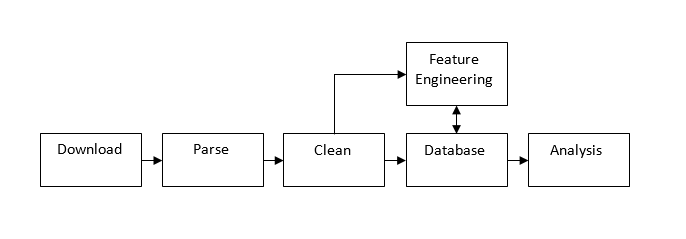
\includegraphics[width=0.7\linewidth]{Figures/FlowChart}
\caption[Flowchart: Data Pipeline]{\small Flowchart of the data pipeline}
\label{fig:pipelineFlowChart}
\end{figure}


%----------------------------------------------------------------------------------------
%	SECTION 1: Raw Data
%----------------------------------------------------------------------------------------

\section{Raw Data} \label{section: Raw Data}

The USPTO offers one of the largest openly available patent networks with images of their patents and trademark documents available since 1796; as text through optical character recognition since 1920 and more recently from 1976 structured full text data (excluding images and diagrams) is available. A subset of the full text data is the bibliographic data; all of the front page information such as date granted, the title of the patent and the citation information. 

This data-set from January 1st 1976 to December 31st 2015 is 110Gb in size in the form of a structured documents of varying formats: From 1976 to 2001 a proprietary text format is used, from 2002 onward the USPTO follows the Patent Grant International Common Element (ICE) document type definition (DTD). While ICE provides international consistency it revised frequently, initially using sgml (ICE 1.5 and 1.6) in 2005 switching to XML for versions 4.0 - 4.4 \cite{ICE}. One patent from each of the three major formats (text, sgml and xml) are included in appendix \ref{AppendixB}, \ref{AppendixC} and \ref{AppendixD} respectively. 

Up until 1996 each year contains one file containing all the patent information in that year in a single document. After this point there is a separate file for each week an associated file listing all the patent numbers present in that file and a summary file containing extra information such as notes about that week and the number of total patents granted of each type. The sgml and xml files have each patent as a single document appended into a single file. 

%-----------------------------------
%	SECTION 2: Parsing
%-----------------------------------
\section{Parsing} \label{section:parsing}

The above structure of the data presents a number of challenges to the parsing process. Most notably the changing formats and schema. The difficulty is parsing these in a consistent way, to minimise any systematic differences between the formats.

A single parsing function for all formats was developed; using the same functional structure to process each format  (Appendix \ref{AppendixA}). The core logical loop for parsing each line of data, shown in figure \ref{fig:FlowChartCoreLogic}, extracts the tag and contents of each line, where the tag is the expression identifying what the contents is, e.g. <date>20011004</date> indicates the contents between the brackets is a date. The function then maps the tag to an action and takes that action. This minimizes differences between formats as long as a semantically equivalent mapping can be found for each. 

The parsing function builds up two tables, one for the patent level data and one for the citations. Initializing each of these as empty vectors, adding patent information and citation information to those vectors and flushing them by appending them to a csv file at the end of each citation or patent section in the document \ref{fig:FlowChartParseStructure}. Some tags are not unique, such as date referring to the date a patent was granted the date a patent application was made or the date a citation patent was granted. To resolve this issue the function identifies the region of a patent document it is currently in and therefore how to interpret uniquely a non-unique tag. It also takes the opportunity to record the degree of each patent with a simple counter. 

The second philosophy of this method of parsing makes it easy to adjust the variables being recorded by adding the tags to the mapping vectors (and name), this flexibility handles changes in schema over time and parsing new variables. 

The variables parsed for each patent were: Patent number, degree, date granted, main and further classification codes. The variables extracted for each citation were: Parent patent number, citation patent number, citation patent granted date, country of the citation and 'cited by' which distinguishes between two classes of individual producing the citation. In this way the citations are in a tall format, in accordance with Hadley Wickham's principles of 'tidy data' \cite{wickham2014tidy}. 

\begin{figure}
\centering
\begin{subfigure}{.3\textwidth}
  \centering
  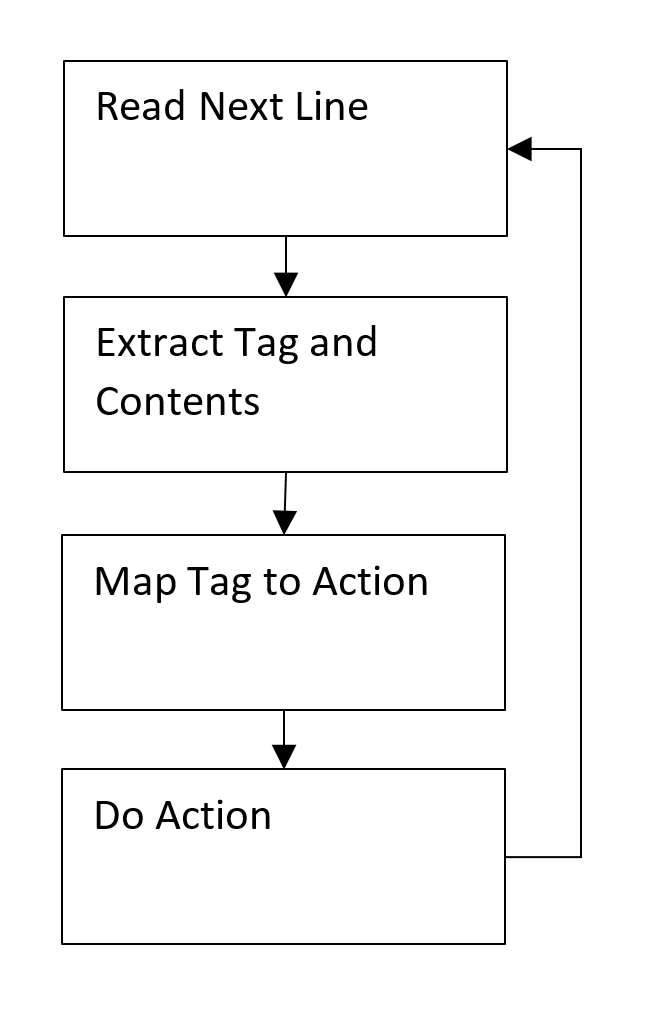
\includegraphics[width=0.7\linewidth]{Figures/FlowChartCoreLogic}
  \caption{}
\label{fig:FlowChartCoreLogic}
\end{subfigure}%
\begin{subfigure}{.7\textwidth}
  \centering
  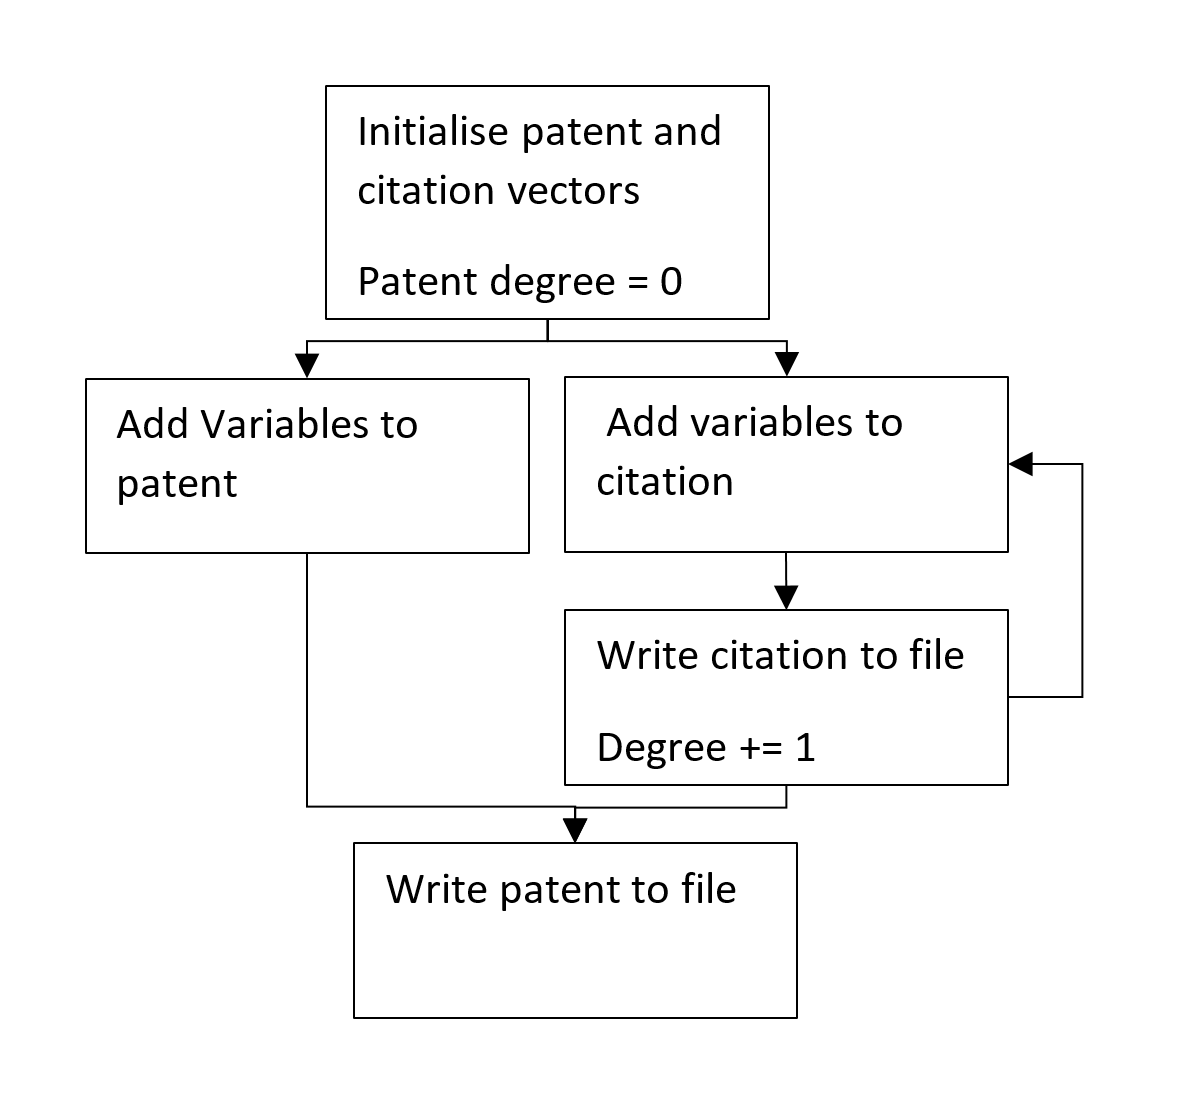
\includegraphics[width=0.7\linewidth]{Figures/FlowChartParseStructure}
  \caption{}
\label{fig:FlowChartParseStructure}
\end{subfigure}
\caption[Flowchart: Parsing Function]{\footnotesize Flowchart showing the structure of the document parsing function. (A) describes the logical loop while (B) describes the structure in which a whole patent is parsed into a patent Vector and a citation table}
\label{fig:Structure of Parsing Algorithm}
\end{figure}

%-----------------------------------
%	SUBSECTION 1: Cleaning
%-----------------------------------

\subsection{Cleaning} \label{section:Cleaning}

After parsing the data it is cleaned to remove some sources of systematic errors. Dealing with big data, considerations must be made when cleaning the data with respect to the impact compared to the difficulty performing that cleaning. The data is tested against some reference points to assess its consistency, both internally between different formats and schema and externally against other sources. 

The categorical factors such as 'citedBy' and 'Country' are cleaned by generating a list of possible values that factor can take and excluding values outside those levels. The dates are in a numeric format "YYYYMMDD" (Where Y,M,D refers to digits representing Year, Month and Day respectively). This is parsed into a date object represented by the number of days since the 1st of January 1970. This allows the dates to be more directly compared as they can be subtracted to get time differences. This process also isolates any values which do not conform to the expected format and returns NA. Using 2001 as an example only 1 date failed to parse this way. Dates on the patents must also in the range of 1976 and 2015. Citation dates can be lower as patents may cite other patents which are not in our data-set. 

Technology codes and patent numbers follow specific schema, US patent numbers are numeric codes which may have a preceding letter (D|RE|PP| H|T) indicating their class, e.g. 'D' represents design patents. While it can be ensured that all US patents use this schema there are foreign patents with many different schema, it is impractical to clean for all these foreign patent schema. In practice not cleaning these foreign patent numbers is unlikely to have an impact on the analysis as the primary purpose for cleaning these patent numbers is to improve matches between citations and patents, which is only necessary for internal citations.  

The patent numbers under citations had several encoding inconsistencies with those under the Patent: punctuation, white-space, additional filler '0' characters and additional digits at the end of the number when parsed from the text format were all cleaned. In 2001 94.5\% of the US citations after 1976 were matched with patents parsed. 

There are a variety of sources of NA values in the dataset. In the parsing phase missing data in the raw dataset is returned as NA and when reading the outputted csv each value must be the expected type (e.g. Order must be an integer). The cleaning phase also produces NA values when a factor value doesn't fit into allowed levels. For example in 2001 4 citations were completely NA, 155 numeric dates are NA and 897 dates when parsed into date format are NA. That year there are a total of 2,609,494 citations so NA values are negligible in quantity. 

The parsed and cleaned data can be compared to those published by the USPTO \cite{USPTOSummary}, as well as the number of patents in the '.lst' files which mirror the raw files documenting the patent numbers present. If accurate, differences between these files and parsed patents represent the patents that the parsing function has failed to process. '.lst' files are only available from 1997 onward (figure \ref{fig:patentCountsTest}). There are two large differences between patent counts at either end of the data-set; in 1976 and 2016. The difference in 2016 is due to two weeks of data having access denied during the download stage but all the weeks are present in 1976 so the difference here is unknown. Due to the relative size of these errors these years have been omitted from patent count based analysis. Before 2008 the number of patents parsed was equivalent to the USPTO summary statistics, since then however the parsed data has significantly more patents than present in the summary statistics. Manually looking up some of these additional patents reveals them to be complete non-duplicated patents so it is not clear why they may be missing. There have always been a small number of patents in the list files not parsed, however until approximately 2010 these numbers were fewer than 100 but have grown to around 1\% of the data, this aligns with the summary statistics divergence suggesting they also experienced these problems to a more severe degree. The difference here doesn't line up with the introduction of XML (2005) but may be due to some of the ICE schema changes or errors in the structure of the document (trying to use an XML parsing library on these years yielded a lot of missing data due to failure to structural errors in the XML). 

\begin{figure}
\centering
\begin{subfigure}{\textwidth}
  \centering
  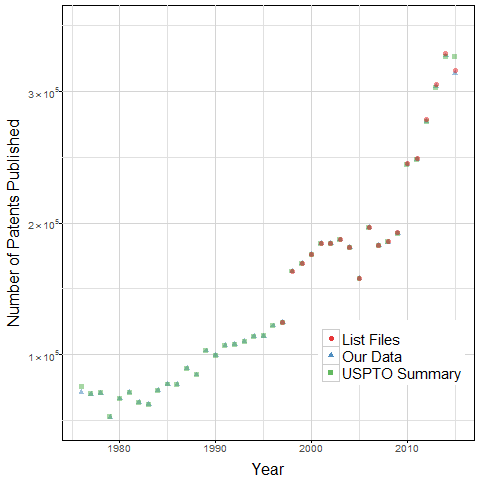
\includegraphics[width=0.9\linewidth]{Figures/patentsCompared}
 \caption{Number of Patents parsed each year from each source}
\label{fig:patentsCompared}
\end{subfigure}%
\\
\begin{subfigure}{\textwidth}
  \centering
  
\includegraphics[width=0.7\linewidth]{Figures/patentsDiff}
  \caption{\footnotesize Difference between number of Patents parsed from different sources and parsed data}
\label{fig:patentsDiff}
\end{subfigure}
\caption[Difference between number of patents parsed from different sources]{\footnotesize The number of Patents granted each year according to 3 sources: Parsed data; a USPTO report and the .lst files.}
\label{fig:patentCountsTest}
\end{figure}

The second reference point for parsing the data is internal consistency. In 2001 both text and sgml data files are present. This gives the unique opportunity to parse both and compare the results. We found that 95 / 184078 patents are present in the text parsing but absent in the sgml, but none are present in the sgml and absent in the text format. Manually referencing the patent numbers with the USPTO database reveals they are valid patents missed absent from the sgml document rather than missed from the parsing method. When these patents are taken into account all citations are present in both formats. Overall these differences confirm that although there are some differences in the raw data, the parsing function is treating differing data formats equally.


%----------------------------------------------------------------------------------------
%	SECTION 3: Database processing
%----------------------------------------------------------------------------------------

\section{Database processing}

Once the data has been parsed and cleaned some analysis can be done on it, but most analysis requires feature engineering. Because the data does not fit in memory this can be done in batch but often the data must be reordered or regrouped, for this reason a database was used. Mongodb was chosen for this as it is designed around big data with its map-reduce and aggregation frameworks making these feature engineering operations to be done in parallel, having javascript and JSON as primary interfaces allowed for ease of use. 

\begin{figure}
\centering
\begin{subfigure}{.5\textwidth}
  \centering
  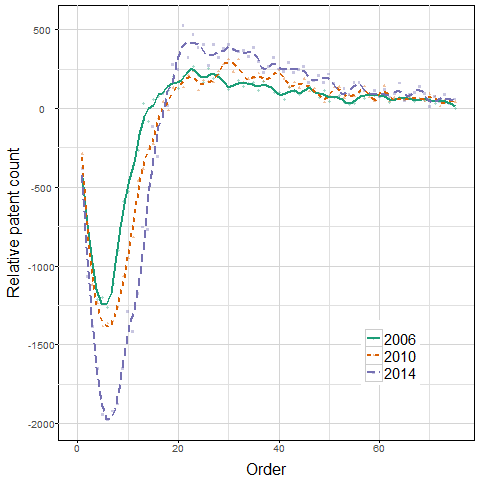
\includegraphics[width=.9\linewidth]{Figures/parsingErrorsPerOrder}
 \caption[]{}
\label{fig:parsingErrorsPerOrder}
\end{subfigure}%
\begin{subfigure}{.5\textwidth}
  \centering
  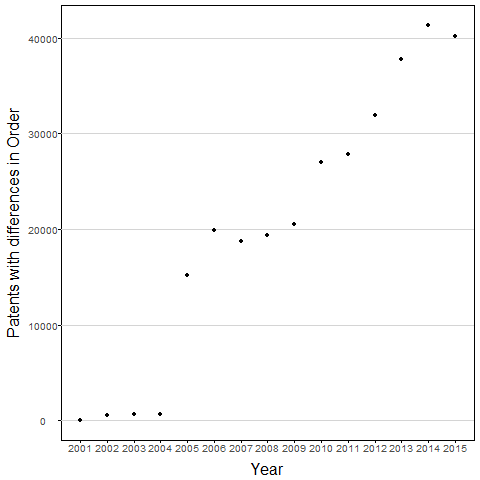
\includegraphics[width=0.9\linewidth]{Figures/parsingErrorsPerYear}
  \caption[]{}
\label{fig:parsingErrorsPerYear}
\end{subfigure}
\caption[Differences in different parsing methods]{Number of patents with different order based on parsing method. (A) against order for the years 2006, 2010 and 2014 and (B) for each year.}
\label{fig:parsingErrors}
\end{figure}

Using a map-reduce the order for each patent was calculated as the number of citations matching each patent. There are some differences between these orders and the ones produced with the parsing function (figure \ref{fig:parsingErrors}).  We can see that these differences are only non-negligible after 2005, when the XML format is introduced. Manual inspection shows that the map-reduced orders are the ones which are incorrect but it is not obvious what the cause of the error is. The map-reduce over represents small orders and under-represents large orders, with the same total number of citations parsed. This suggests that the map-reduce may be interpreting a single patent as multiple different patents. This error only becomes significant in the most recent years but represents 1\% of the data in 2015, so caution is advised for these years. 

In summary the parsing and cleaning of the data have focused heavily on maximizing the consistency of the data parsed from the design of the parsing function to the cleaning steps. We have analysed these results and find that it out-performs USPTO summary statistics and non-negligible errors appear to be limited to 1976 and the last few years of the data-set. It is important to know where these errors are and be cautious when analysing them but we can't dismiss these sections of the data-set. 
% Chapter Template
\chapter{Analysis} % Main chapter title

\label{Chapter4} % Change X to a consecutive number; for referencing this chapter elsewhere, use \ref{ChapterX}

\section{Data Summary} \label{Data Summary}

After parsing and cleaning the data is stored in two tables, a patent table and a citation table as shown in tables \ref{tab:patents} and \ref{tab:citations}. Definitions of variables are described in section \ref{section:Cleaning}.

The dataset covers the time period from 1976 to 2015, over this period 5,803,302 patents have been processed along with 114,585,378 citations. Since 2001 where the data dictating who cited each citation was initially released 25.7\% of citations have been the Examiner and the rest being other sources. Since 2005 where accurate country codes for foreign patents have been released 85.5\% of citations have been internal, i.e. to other US patents.

\begin{table}[ht]
\caption{First 6 entries in parsed and cleaned patent table, 1976}
\label{tab:patents}
\centering
\begin{tabular}{rlrrr}
  \hline
 & Patent & Date & Order & Date2 \\ 
  \hline
  1 & RE28671 & 19760106 &   8 & 2196 \\ 
  2 & RE28672 & 19760106 &   7 & 2196 \\ 
  3 & RE28673 & 19760106 &   3 & 2196 \\ 
  4 & RE28674 & 19760106 &   5 & 2196 \\ 
  5 & RE28675 & 19760106 &  13 & 2196 \\ 
  6 & 3930271 & 19760106 &   2 & 2196 \\ 
   \hline
\end{tabular}
\end{table}

\begin{table}[ht]
\caption{First 6 entries in parsed and cleaned citation table}
\label{tab:citations}
\centering
\begin{tabular}{rllrllr}
  \hline
 & Patent & Citation & Date & CitedBy & Country & Date2 \\ 
  \hline
1 & D607176 & 534632 & 18950200 & cited by examiner & US & -27362 \\ 
  2 & D607176 & D28957 & 18980600 & cited by other & US & -26146 \\ 
  3 & D607176 & D45899 & 19140600 & cited by other & US & -20303 \\ 
  4 & D607176 & D59909 & 19211200 & cited by examiner & US & -17563 \\ 
  5 & D607176 & D96223 & 19350700 & cited by examiner & US & -12603 \\ 
  6 & D607176 & D96224 & 19350700 & cited by examiner & US & -12603 \\ 
   \hline
\end{tabular}
\end{table} 
%----------------------------------------------------------------------------------------
%	SECTION 1: Patents per Year
%----------------------------------------------------------------------------------------
\section{Network Summary} \label{Network Summary}

In this section some general summaries of the network are computed. Some of these summaries have been previously carried out by other authors allowing validation of this/their analysis. 

%-----------------------------------
%	SUBSECTION 1: Cumulative distribution 
%-----------------------------------

\subsection{Patents per Year} \label{Patents per Year}

\begin{figure}
\centering
 \centering
 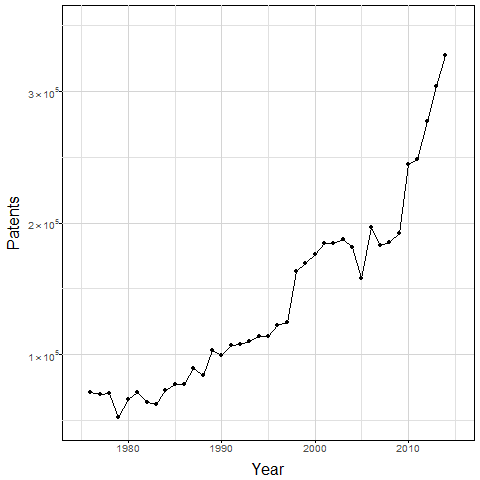
\includegraphics[width=0.7\linewidth]{Figures/PatentCountVsYear}
\caption[Number of patents granted each year]{Number of patents granted each year from 1976 to 2014}
\label{fig:PatentCountVsYear}
\end{figure}

Each patent was grouped by the year in which it was published and frequency computed. The year 2015 was omitted due to the presence of two missing months of data due to a download error on the part of the USPTO as discussed in the previous section. 

Figure \ref{fig:PatentCountVsYear} shows the number of patents granted each year on linear scales. There are two main features: a large jump between 1997 and 1998 and a transition to very rapid growth after 2009. Note that these events don't align themselves with changes in the data format which occur from 2001-2002 and from 2004-2005. This transition may be caused by socio-economic or political effects as it occurs directly after the 2008 recession, regardless the continued growth after 2009 indicates a change in the evolution of the network. Valverde et al. \cite{valverde2007topology} conducts a similar analysis, over the years of 1986 to 2005, which has the same general shape but some minor differences; most visibly in the size of the gap between 1997 and 1998 which is bigger in this analysis than the former. In the previous chapter patent counts per year were compared to other sources, USPTO summary statistics and the 'lst' files, consistency of these points to some possible difference in methodology or parsing errors in the case of Valverde's paper. 

Valverde et al. claims that this metric of patents granted per year follows a power law distribution. To demonstrate this they plot the cumulative number of patents on log-log scales and make a linear fit. To replicate this analysis patent counts per year the cumulative number of patents in the network is computed and plotted on logarithmic scales. A generalised linear model is fitted using least squares regression and a log-log transform. 

Figure \ref{fig:CumPatents2} shows the cumulative number of patents granted over time starting in 1976 and ending in 2014. Time is given as number of years from the origin. Figure (A) shows a power-law model fitted to the entire dataset and its exponent whereas figure (B) conducts this method only on the years 1986 to 2005. The cumulative distribution is often used to identify power-law behaviour because often the tail of the distribution has rare events with large amounts of statistical noise, the cumulative integrates the noise into a smooth function. If $ p(x) = x^{\alpha}$ the cumulative distribution is also a power law with smaller exponent:

$$ P(x) =  \frac{1}{\alpha - 1}x^{(\alpha - 1)}$$

While not necessary in this instance due to the absence of a noisy tail, a CDF was used to closely replicate the Valverde methodology and is general best practice. Although using least squares regression on a log-log transformed cumulative distribution is not the most rigorous method for fitting power-law distributions introducing small bias to the exponent, this appears to be the methodology used in the Valverde paper (although it is not clear) additionally the exact value of the exponent is not important only the general shape of the model. 


\begin{figure}
\centering
\begin{subfigure}{.5\textwidth}
  \centering
  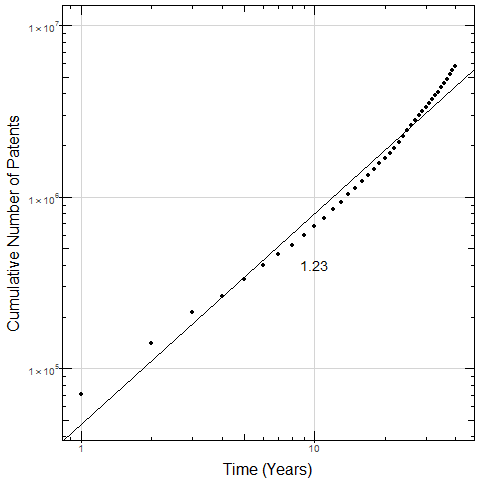
\includegraphics[width=0.7\linewidth]{Figures/CumulativePatents1}
 \caption[CumPatents1]{\small}
\label{fig:CumPatents1}
\end{subfigure}%
\begin{subfigure}{.5\textwidth}
  \centering
  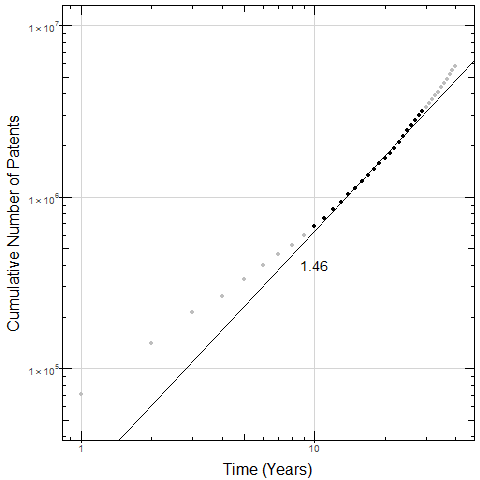
\includegraphics[width=0.7\linewidth]{Figures/CumulativePatents2}
  \caption[CumPatents1]{\small G}
\label{fig:CumPatents2}
\end{subfigure}
\caption[Power-law fit for cumulative number of patents granted each year]{The cumulative number of patents granted from 1976 to 2015, plotted on a log-log scales. Fitted with generalised linear model of the form $y = x^{\alpha}$ using (A) all the data and (B) only the data in over the years 1986 to 2005.}
\label{fig:CumPatents}
\end{figure}

From \ref{fig:CumPatents1} there is a clear divergence from the fit over the first few years. In Valverde's paper it appears that in their paper they may have disregarded these first few points as outliers, this can be shown by figure \ref{fig:CumPatents2} which omits these points yielding a very similar exponent (1.46 vs. 1.45). Since 2005 where their data-set ended new data-points do not fit this model well. This is more apparent in figure \ref{fig:patentCountFit} which shows this same fit on the non-cumulative plot. 

Using the same methodology as before an exponential fit to the data is produced, \ref{tab:distributions}. This is shown on figure \ref{fig:cumulativePatentFits} with a 95\% confidence interval along side the original power-law fit. 

\begin{figure}
\centering
\begin{subfigure}{.3\linewidth}
  \centering
  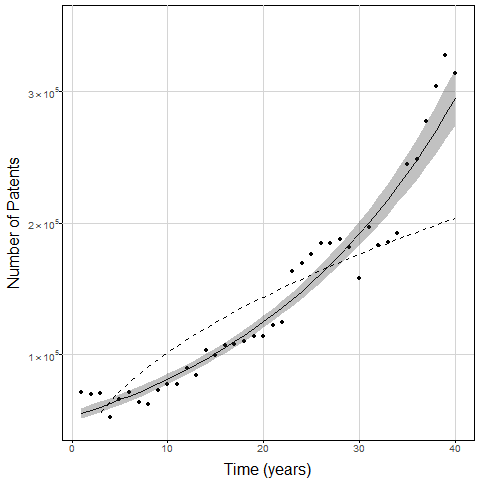
\includegraphics[width=0.9\linewidth]{Figures/patentCountFit}
 \caption[CumPatents1]{\footnotesize Patents granted per year}
\label{fig:patentCountFit}
\end{subfigure}%
\begin{subfigure}{.3\linewidth}
  \centering
  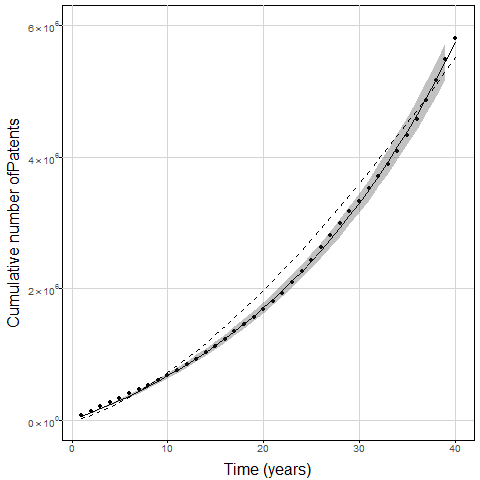
\includegraphics[width=0.9\linewidth]{Figures/patentCountFit_cum}
  \caption[CumPatents1]{\footnotesize Cumulative number of patents granted}
\label{fig:patentCountFit_cum}
\end{subfigure}
\begin{subfigure}{.3\linewidth}
  \centering
  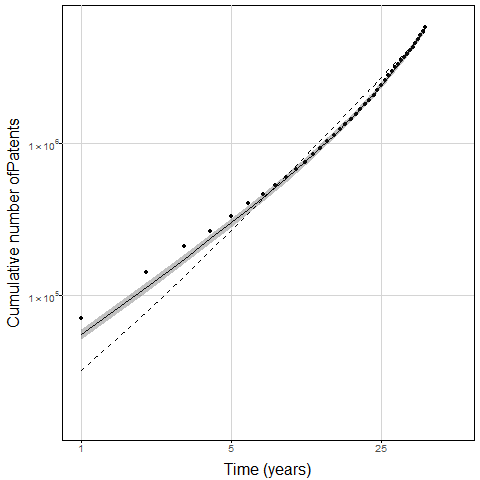
\includegraphics[width=0.9\linewidth]{Figures/patentCountFit_cum_loglog}
  \caption[CumPatents1]{\footnotesize Cumulative patents granted on a log-log scale}
\label{fig:patentCountFit_cum_loglog}
\end{subfigure}
\caption[Exponential fit for number of patents granted each year]{Power law and exponential fits for cumulative number of patents published each year}
\label{fig:cumulativePatentFits}
\end{figure}

It is clear that a power-law fit doesn't fit the data, it is plausible that an exponential model may be more accurate (fig.\ref{fig:cumulativePatentFits}). However the presence of two major shifts in the distribution in 1997/8 and 2009/10 indicate that large external effects are causing changes in this data-set. These changes are significant enough that without taking them into account or aggregating over a longer period of time or smaller timescales making a statistically significant claim about the underlying distribution here would be difficult.  

%-----------------------------------
%	SUBSECTION 1: Cumulative distribution 
%-----------------------------------


\subsection{Degree Distribution} \label{Degree Distribution}

The degree distribution is the frequency distribution of patents with respect to the total number of citations they make. It can inform how new citations are made and copes well with the evolution of the network over time as analysing years separately they do not need to be normalised. This has been separated into different years and the years 1984,1992, 2002 and 2012 have been on a log-log scale and fitted with a generalised linear model as before to replicate the third plot in the Valverde paper \ref{fig:OrderDistribution}. 

The exponent of the power-law is increasing over time, indicating both more citations over time but more extreme values also. These values however are quite different from those found by Valverde who found an exponent of -4.0 in 2002. This may be due to a number of methodology differences, most likely that our analysis includes foreign patents. We see that the frequency increases to a peak giving the distributions a mode of 6 to 8 depending on year, after around 10 to 20 this appears to converge to a power law.

\begin{figure}
\centering
  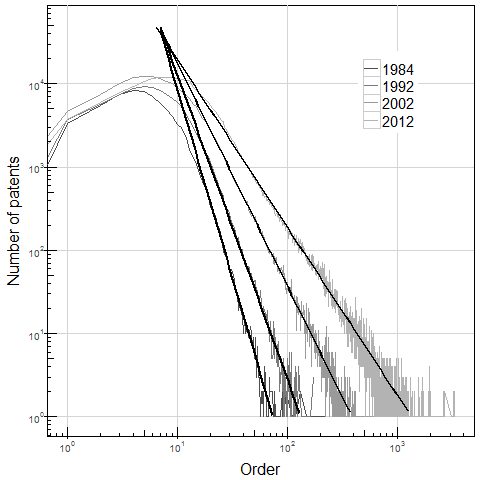
\includegraphics[width=0.7\linewidth]{Figures/OrderDistribution}
  \caption[Degree Distribution]{Degree distribution (number of citations for each patent) on a log-log scale shown for years 1984,1992,2002,2012. Fit with generalized linear model of the form $y \sim x^\alpha$ yielding exponents of minus 6.31, 6.92, 7.77 and 8.46 respectively}
\label{fig:OrderDistribution}
\end{figure}

As before some best practices have been ignored in order to reproduce the Valverde et al. paper better. Valverde claims that this distribution follows an extended power law of the form $ P(k) \sim (k + k_0)^{-\gamma} $, where $k$ is the degree and $k_0$ and $\gamma$ are constants. An extended power-law  converges to a power law of $k >> k_0$ and converges to an exponential for $ k << k_0$, it is therefore functionally similar to the popular model of a power-law with an exponential cut-off. They do not however state how they make their fit or conduct any tests to identify the efficacy of such a fit. 

Considering the 4 different years presented in figure \ref{fig:OrderDistribution} and the 4 most popular discrete distributions described in table \ref{tab:distributionsP}, each of these functional forms is fitted to the cumulative frequency order distribution by maximising their likelihood functions. The cumulative distribution is used as it mitigates noise caused by low frequency events. This is done while optimising the cut-off value $x_{min}$ for that distribution. Optimising $x_{min}$ uses a method proposed by Clauset et al. which searches over a range of values and minimises the difference in probability distributions of the data and the fit \cite{clauset2007frequency}. The difference metric used is the Kolmogorov-Smirnov statistic; the maximum distance between the two distributions. 

The accuracy of these fits is assessed using a bootstrapping algorithm, the distribution is sampled with replacement $n$ times, each time the KS statistic is computed between this sampled distribution and the original data. The P value is given as the proportion of sample distributions less similar to the original distribution than the fit. A rule of thumb given by Clauset et al. states to achieve an error of approximately $\epsilon$ the number of samples used should be at least $\frac{1}{4}\epsilon^{-2}$. 2500 samples were used to achieve $\epsilon \approx 0.01$ \cite{clauset2009power}. 

From figure \ref{fig:distributionFits} we see the increasing gradient of the power-law exponent over time, additionally the distribution appears to become less straight and has greater changes in shape at the tail, which was harder to identify using the non-cumulative plot \ref{fig:OrderDistribution}. As the distribution becomes less straight the power-law fit becomes less accurate especially failing to capture the shape of the tail. The Poisson and exponential distribution never successfully fit the main body of the data, the Poisson distribution especially fails in this regard fitting either poorly in 1984 or to increasingly small subsections of the tail in later years. The exponential function follows a similar trend, fitting the main body of the data poorly initially before trying to fit only the tail of the distribution, matching the exponential with the power-law suggests that an exponential cut-off is plausible however the log-normal distribution also appears to be a good fit, capturing some of the behaviour of the tail in a way none of the other distributions were able to. 

\begin{table}
\caption{Functional form and maximum likelihood estimate (MLE) of distributions tested}
\label{tab:distributions}
\centering
\begin{tabular}{l l l}
\toprule
Distribution & $f(x)$ & MLE\\
\midrule
Power Law & $ x^{-\alpha}$ & $ \hat{\alpha} = 1 + n[\sum^n_{i=1}ln\frac{x_i}{x_{min}}]^{-1} $ \\
Log-Normal & $\frac{1}{x}exp[-\frac{(lnx-\mu)^2}{2\sigma^2}] $  & $ \hat{\mu} = \frac{\sum lnx}{n}, \hat{\sigma^2} = \frac{\sum_k(lnx_k - \mu)^2}{n} $ \\
Exponential & $ \exp^{-\lambda x}$  & $\hat{\lambda} = \frac{1}{\bar{x}} $ \\
Poisson & $ \frac{\lambda^x\exp^{-\lambda}}{x!}$ & $\hat{\lambda} = {\sum^n_{i=1}k_i}{n} $ \\ 
\bottomrule\\
\end{tabular}
\end{table}

\begin{figure}
\centering
  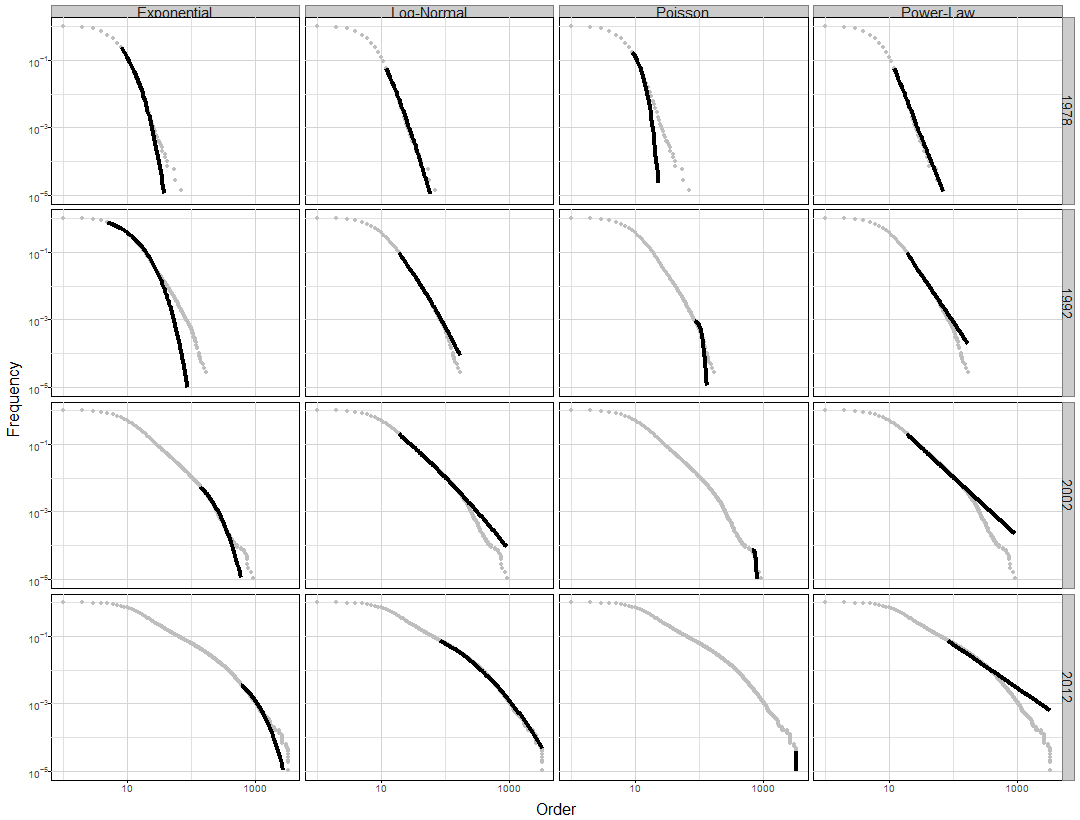
\includegraphics[width=\linewidth]{Figures/distributionFits}
  \caption[]{Cumulative density function fitted using maximum likelihood estimates for Poisson, Exponential, Log-normal and Power-law distributions}
\label{fig:distributionFits}
\end{figure}

\begin{table}
\caption{P values fitting distributions to the degree distribution obtained through bootstrapping method on a n = 10000 sample of the data}
\label{tab:distributionsP}
\centering
\begin{tabular}{l l l l l}
\toprule
Year & Power-Law & Log-Normal & Poisson & Exponential \\
\midrule
1984 & 0.494 & 0.302 & 0.000 & 0.001 \\
1992 & 0.820 & 0.934 & 0.000 & 0.005 \\
2002 & 0.534 & 0.399 & 0.108 & 0.000 \\
2012 & 0.266 & 0.280 & 0.000 & 0.448 \\
\bottomrule\\
\end{tabular}
\end{table}

Note that this bootstrapping procedure is conducted on a sample of 1000 observations due to heavy performance issues with the algorithm while the distribution fits use the entire dataset, this can lead to large differences between the two as different $x_{min}$ values are optimised. For example in 2002 and 2012 the Poisson distribution has a very large $x_{min}$ and therefore a higher p value would be expected than when it poorly fits to the whole curve. While the small sample size relative to the size of the data may limit the insight from this test, the consistently low and often 0 values of the Poisson and Exponential distributions means they can likely be dismissed as candidates for this distribution. 

While the power-law and log-normal distributions are consistently significant it is not sufficient to say that the power-law is better than the log-normal. To compare the models directly Vuong's test is used \cite{vuong1989likelihood}, this is based on the null hypothesis that both fits are equally far from the true distribution, if true the log-likelihood is expected to have a Normal distribution. This test is done using the complete data (without sampling) using the fits shown in figure \ref{fig:cumulativePatentFits}. 

\begin{table}
\caption{P values giving upper limit of if power-law is true (one-sided) or both power-law and log-normal distributions are equally good (two-sided) using Vuong's test}
\label{tab:Vuong}
\centering
\begin{tabular}{l l l}
\toprule
Year & One-sided & Two-sided \\
\midrule
1984 & 3.87e-1 & 7.74e-1  \\
1992 & 1.39e-4 & 2.78e-4  \\
2002 & 1.1e-10 & 2.3e-10  \\
2012 & 9.3e-86 & 1.9e-85  \\
\bottomrule\\
\end{tabular}
\end{table}

The power law is never the more likely distribution based on this test but in 1984 it is significant to the degree that the two-sided test, indicating both distributions are equally likely has high p-value. However this likelihood of a power law being true consistently decreases over time so that in 2012 there is a $9.3 \times 10^{-86}$ chance of a power-law in contrast to the log-normal distribution. 

%----------------------------------------------------------------------------------------
%	SECTION 1
%----------------------------------------------------------------------------------------

\section{Coloured Network Analysis} \label{Coloured Network Analysis}

One of the features parsed was who contributed the citation to the patent document. From 2001 to 2013 this is split into two categories "Cited by Examiner" and "Cited by Other". The Examiner has a duty to fulfil the legal requirements of the patent application citing any prior art which was absent from the patent previously. Cited by Other "indicates those cited in a protest, by an attorney or agent not acting in a representative capacity but on behalf of a single inventor, and by the applicant" \cite{USPTOSummary}. In reality all sources of citation besides the applicant are rate, this is shown in 2014 and 2015 where the 'cited by other' field was split into two, 'cited by applicant' and 'cited by third party'. Over these two years 99.999\% of these citations were 'cited by applicant' rather than the third party. For the sake of consistent analysis these have been combined again into a 'cited by other' category.

This 'citedBy' field was analysed because of the differing motivations and responsibilities of the parties involved. The Examiner with a legal and professional responsibility is likely to act differently from the applicant and many of the features that make the patent network unique are the legal responsibilities that citations have so studying this sub-network could yield more varied results than the network as a whole, especially when compared to other bibliographic networks. 

\subsection{Degree Distribution}
The degree distribution of for the two sub-networks are calculated in the same way as section \ref{Degree Distribution} shown in figure \ref{fig:orderDistributionCitedBy} and the mean degree for each of the two sub-networks and total are calculated for each year \ref{fig:av_degree_vs_year}.

\begin{figure}
\centering
\begin{subfigure}{\textwidth}
  \centering
  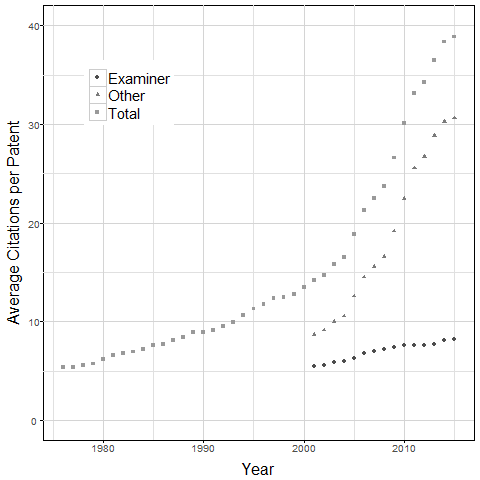
\includegraphics[width=0.7\linewidth]{Figures/av_degree_vs_year}
 \caption[]{\small Average degree by citedBy for the years 2001 to 2015 and average total degree from 1976 to 2015}
\label{fig:av_degree_vs_year}
\end{subfigure}%

\begin{subfigure}{\textwidth}
  \centering
  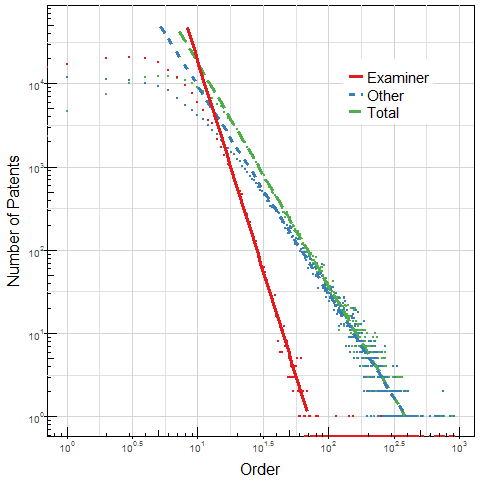
\includegraphics[width=0.7\linewidth]{Figures/orderDistributionCitedBy}
  \caption[]{\small Degree distribution by citedBy on a log-log scale, fitted with generalised linear model of the form $y \sim x^{-\alpha}$, here total refers only to the years 2001 to 2015}
\label{fig:orderDistributionCitedBy}
\end{subfigure}
\caption[]{}
\label{fig:degreeCitedBy}
\end{figure}

The average number of citations for each patent changes very little over time for the Examiners but increases rapidly over the available data range for 'Other'. As Other dominates the Examiner the total value follows this closely this means that the structure of the Examiner network is masked. It is unclear how this relationship held over the previous years, it may be that the two sources of citation had a more harmonious relationship in the past as over the period of time from 1976 to 200 the increase in average citation over time is fairly constant and similar to the increase in time of the Examiner network. 

The exponent for the degree distribution is more negative for the examiner indicating that it operates over a smaller range of values, reaching a maximum at approximates 100 rather than 1000. The Examiner distribution also appears to be a better fit in the tail of the distribution and has higher frequencies at low citation counts. 

All of these features of the Examiner network relative to the Other network are not unexpected as they indicate more conservative and consistent practices which would be fairly typical of a professional. The large range of values may suggest a tendency for the applicants to occasionally over-cite their patents to an extreme. 

The changes in average citation number being caused by differences only in the applicants activity could damage the idea that there is a structure of innovation itself over this time period because it suggests that the patents themselves aren't necessarily becoming more interdependent as an increase in average citations per patent otherwise suggests. However this doesn't discount the idea as the Examiner acts after the applicant so changes to the patents/innovations themselves could be accounted for by their actions alone although this is a less likely explanation. 

%----------------------------------------------------------------------------------------
%	SECTION 2
%----------------------------------------------------------------------------------------

\subsection{Correlation} \label{Correlation}

In order to investigate the relationship between the Examiner citations and Other citations a number of analyses of correlation between the order of each is measured (number of Examiner citations vs. number of Other citations for each patent). 

A scatter-plot of all patents from 2001 to 2015 was made using a log-log scale, comparing the number of citations made by Examiners to those made by Others, because these orders are discrete a uniform random noise of $\pm 0.5$, this expands the data to uniformly occupy the area which rounds to its discrete value. This allows the density to be seen more clearly. The scatter-plot is made with a sample of 100,000 observations and a linear fit is added using least square regression to represent the correlation between the two. 

To more clearly represent the density of the scatter-plot a contour density graph is built on a log-log scale using two-dimensional kernel density estimation. This evaluates a bivariate normal kernel over the log-log transformed data to produce a density estimate. This is done without the random uniform noise because the discrete density is well represented already. The bandwidth of the kernel for a data vector $x$ is the normal reference bandwidth given by equation \ref{eq:bandwidth} \cite[page 130]{venables2013modern}: 

\begin{align} \label{eq:bandwidth}
\begin{split}
a &= \frac{Q_3(x) - Q_1(x)}{1.34} \\
b &= \sqrt[]{\sigma_x} \\
bandwidth &= 4 \times 1.06 \times min(a,b) \times N_x^{-1/5} 
\end{split}
\end{align}

The mean and median of one class is computed for logarithmically binned intervals of the other class. I.e. for the set of observations with Examiner degree in the first interval the mean and standard deviation of the Other degree is calculated (figure \ref{fig:MeanOtherVsExaminer}) as well as median and interquartile range (figure \ref{fig:MedianOtherVsExaminer}). The median is computed because heavy tailed distributions can be biassed using the mean and standard deviation only represents error (when transformed to standard error) under the assumption of a normal distribution. 

Finally correlation metrics are computed with p-values using the fBasics R package \cite{fBasics}. Pearson correlation is computed non-parametrically using a bootstrapping procedure. As Pearson correlation is a measure of linear correlation between variables a log-log transformed version was also computed. Kendall's Tau and Spearman's rho are rank based measures so work on non-parametric data natively, this means that the rho and the tau are not measures of a linear relationship like the Pearson product-moment correlation. 

\begin{figure}
\centering
\begin{subfigure}{\textwidth}
  \centering
  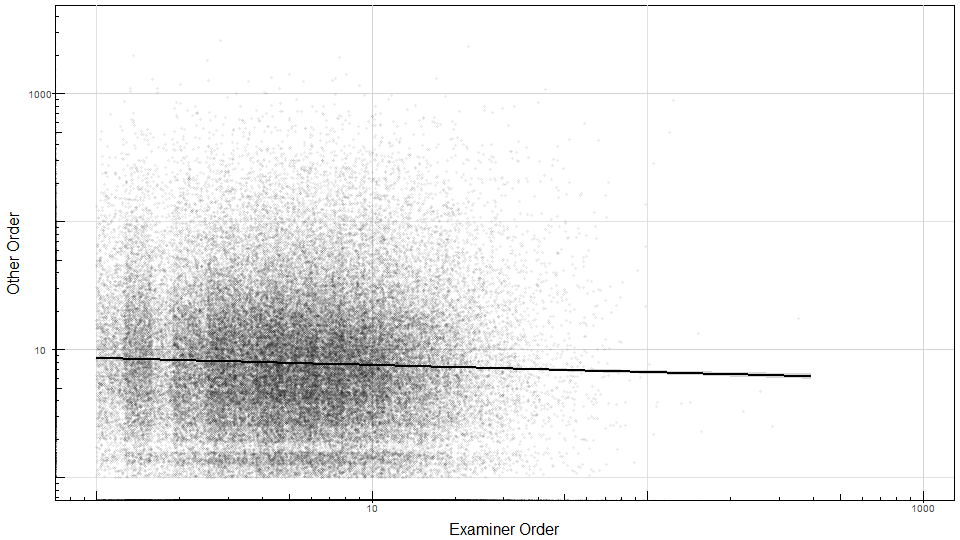
\includegraphics[width=0.9\linewidth]{Figures/orderScatterplot}
 \caption[]{\small Using log-log scale, linear fit shown \newline}
\label{fig:orderScatterplot}
\end{subfigure}%

\begin{subfigure}{\textwidth}
  \centering
  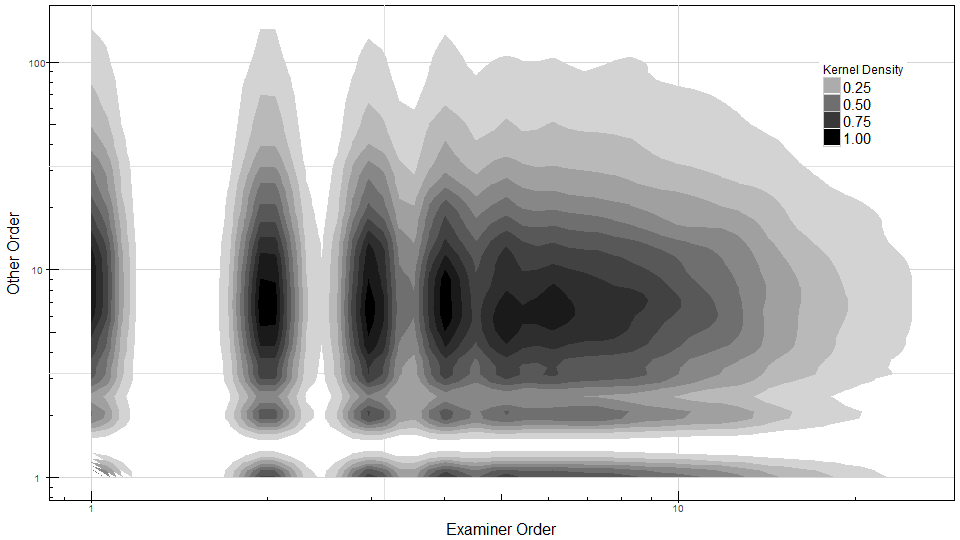
\includegraphics[width=0.9\linewidth]{Figures/orderScatterplotContours}
  \caption[]{\small Contour density graph using Kernel Density Estimator}
\label{fig:orderScatterplotContours}
\end{subfigure}
\caption[Scatterplot of Order for 'Other' and 'Examiner' sub-graphs]{Scatterplot of 'Examiner' and 'Other' orders for each patent using an n = 100,000 sample.}
\label{fig:scatterplots}
\end{figure}

In figures \ref{fig:orderScatterplot} and \ref{fig:orderScatterplotContours} it is clear that any correlation between the two orders are very small in nature, this is supported by all the correlation metrics computed (table \ref{tab:cor}). This is fairly unexpected, under a model that each patent has some underlying true number of citations and applicants have some fairly constant level of completeness for this true number that the correlation would be significant and positive as the greater true citation number the greater the number of citations from both examiner and applicant in this model. However under a model where the true number of citations is fairly constant but the distribution of completeness from the applicant varies a negative correlation would be expected because as the applicant finds most the relevant citations there are fewer left for the examiner to complete the patent. This model however assumes that both the examiner and the applicant are getting citations from a limited set of correct citations, if either is making a significant portion of their citations from outside this set then correlations would decrease. This is likely what is occurring either some of the parties are making citations from outside the set of correct citations and/or the set is not well defined. 

The data may support these models of correlation however, figure \ref{fig:MeanExaminerVsOther} shows a slight negative correlation for the bulk of the data but a positive correlation for the large order values and each of the correlation metrics are slightly negative. Figure \ref{fig:MeanExaminerVsOther} shows that extreme values have slightly positive correlation, while the error is large enough that this effect isn't statistically significant and the discrete nature of the median makes it difficult to identify trends in the other plots, the Kernal density plot does appear to corroborate this slight positive correlation for extreme orders. The Mean of the other for binned Examiner shows a similar effect but the positive correlation peaks before decreasing again, there are  very low sample sizes for these high values of Examiner. 

\begin{figure}
\centering
\begin{subfigure}{0.6\linewidth}
  \centering
  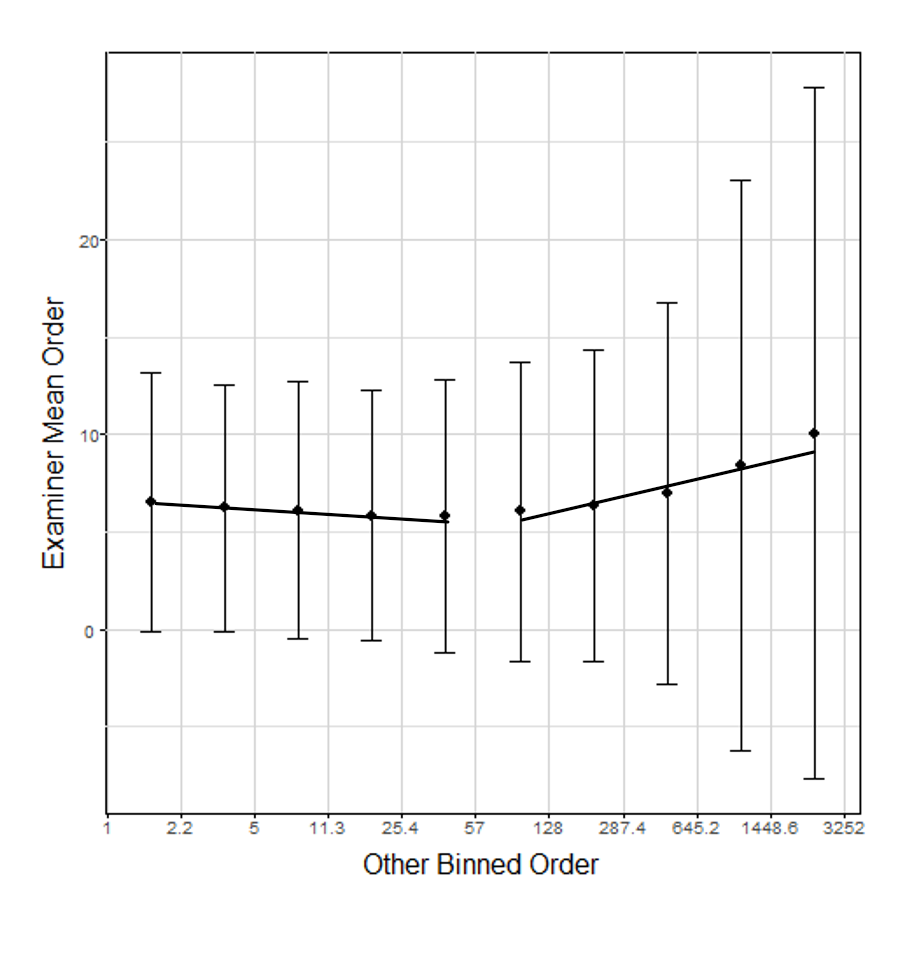
\includegraphics[width=0.9\linewidth]{Figures/MeanExaminerVsOther}
  \caption[]{\small Mean Examiner for Binned Other with two linear regressions over the first 5 bins and last 5 bins.}
\label{fig:MeanExaminerVsOther}
\end{subfigure}

\begin{subfigure}{.24\linewidth}
  \centering
  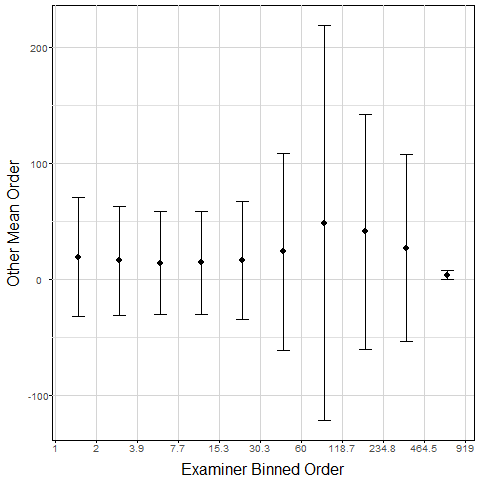
\includegraphics[width=0.9\linewidth]{Figures/MeanOtherVsExaminer}
 \caption[]{\small Mean Other for Binned Examiner\newline}
\label{fig:MeanOtherVsExaminer}
\end{subfigure}%
\begin{subfigure}{.24\linewidth}
  \centering
  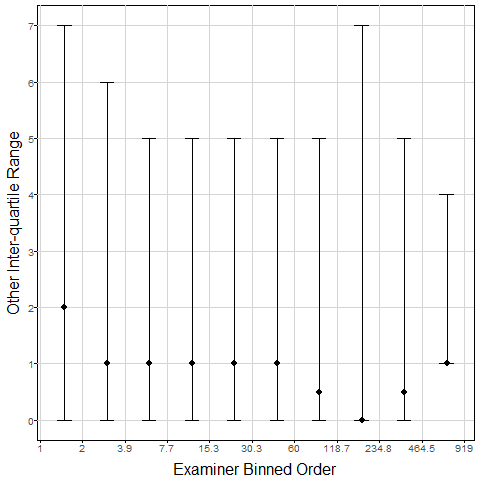
\includegraphics[width=0.9\linewidth]{Figures/MedianOtherVsExaminer}
  \caption[]{\small Median Other for Binned Examiner }
\label{fig:MedianOtherVsExaminer}
\end{subfigure}
\begin{subfigure}{.24\linewidth}
  \centering
  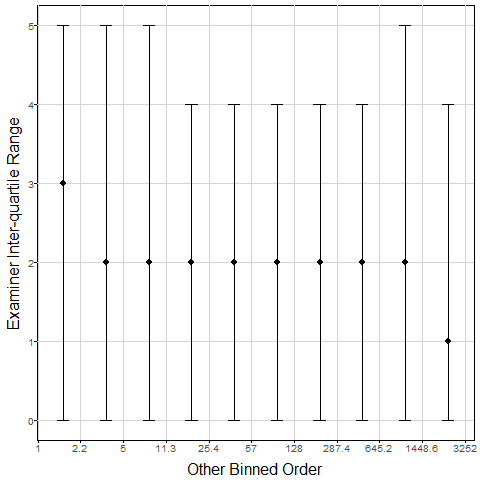
\includegraphics[width=0.9\linewidth]{Figures/MedianExaminerVsOther}
  \caption[]{\small Median examiner for binned Other}
\label{fig:MedianExaminerVsOther}
\end{subfigure}
\caption[]{Comparison of 'Other' and 'Examiner' sub-graphs degree correlation by logarithmically binning one and calculating metrics about the other (mean/median) }
\label{fig:binnedAverageComparison}
\end{figure}

\begin{table}
\caption{Correlation metrics and their P values. Pearson transformed refers to Pearson correlation conducted on log-log transformed data}
\label{tab:cor}
\centering
\begin{tabular}{l l l l}
\toprule
Statistic & Value & One-sided (Less) & Two-sided \\
\midrule
Kendall's Tau & -0.0889 & 2.2e-16 & 2.2e-16 \\
Pearson Correlation & -0.008 & 5.5e-3 & 1.1e-2 \\
Pearson transformed & -0.0378 & 2.2e-16 & 2.2e-16  \\
Spearman's rho & -0.1243 & 2.2e-16 & 2.2e-16 \\
\bottomrule\\
\end{tabular}
\end{table}

%----------------------------------------------------------------------------------------
%	SECTION 2
%----------------------------------------------------------------------------------------

\subsection{Fitting Distributions} \label{section: Fitting Distributions}

As in section \ref{Degree Distribution} four different functional forms are fitted to the cumulative degree distribution using maximum likelihood estimators while optimising $x_{min}$ to minimise the Kolmogorov-Smirnov statistic as a measure of goodness-of-fit. Here the year 2002 is used as a year present in the Valverde analysis which has Examiner and Other networks analysable. A bootstrapping method using 2500 samples to compute a P value to an approximate accuracy of 0.1 is used using the same methods as previously. This method is conducted on a sample of 10000 observations due to the performance limitations of the method. Due to this sample being a relatively small subset of the data results from this are taken with caution. A log-likelihood ratio test is also used to compare distributions, this uses all the available data rather than a sample but first refits the distributions so that both fits share the same $x_{min}$, this is done by setting the $x_{min}$ as the greater of the two previous fits, as it is more conservative, before solving for the other parameter(s) by maximising the likelihood function. 

\begin{figure}
\centering
  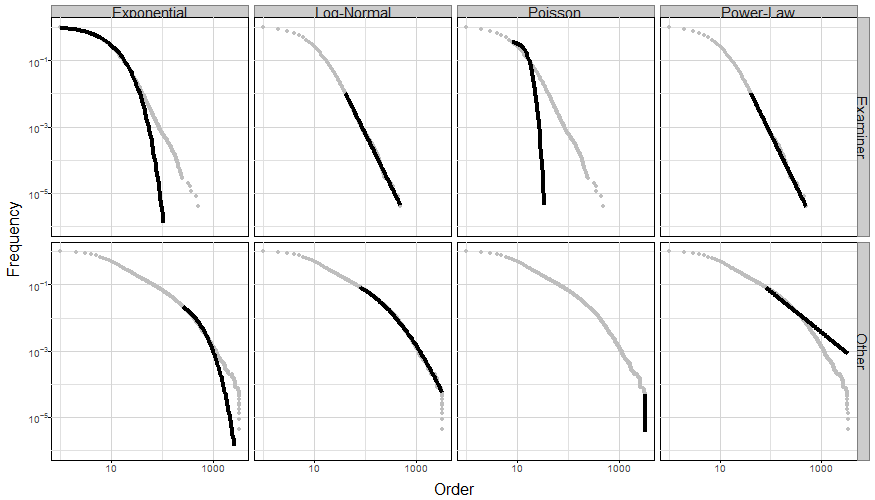
\includegraphics[width=0.7\linewidth]{Figures/ExaminerOtherDistributionFit}
  \caption[Fitting Degree Distribution for "Examiner" and "Other" sub-graphs]{Fitted 2002 degree distributions for "Other" and "Examiner" sub-graphs using Maximum Likelihood for discrete distributions: Poisson, Exponential, Log-normal, Power-law.}
\label{fig:ExaminerOtherDistributionFit}
\end{figure}

\begin{table}
\caption{P values fitting distributions to the degree distribution obtained through bootstrapping method on a n = 10000 sample of the data}
\label{tab:distributionsColouredP}
\centering
\begin{tabular}{l l l l l}
\toprule
CitedBy & Power-Law & Log-Normal & Poisson & Exponential \\
\midrule
Examiner & 0.177 & 0.024 & 0.000 & 0.090 \\
Other & 0.343 & 0.327 & 0.037 & 0.000 \\
\bottomrule\\
\end{tabular}
\end{table}

\begin{table}
\caption{P values for likelihood data is power law distributed in comparison to log-normal using likelihood ratio test}
\label{tab:distributionsColouredP2}
\centering
\begin{tabular}{l l l l}
\toprule
CitedBy & Log Likelihood Ratio & P: One sided & P: Two Sided \\
\midrule
Examiner & 0.352 & 0.637 & 0.725 \\
Other & -14.78 &9.75e-50 & 1.95e-49 \\
\bottomrule\\
\end{tabular}
\end{table}

As in section \ref{Degree Distribution} a P value of less than 0.1 is taken as a rule of thumb to be discounted. Here all the P values are significantly lower than before and none of the Poisson or Exponential distributions get a significant result. While the Other network shows very similar P values for Power-Law and Log-Normal the Examiner network has very low values for the Log-Normal, lower than the Exponential and lower than the threshold for significance. When using the log-likelihood ratio test to compare distributions however the Examiner gives a high 2 sided P value. The two sided test indicates the probability that the data comes from both distributions i.e. that they are both good fits to the data and can't be analytically distinguished. This is in conflict with the bootstrapping results although as previously stated the small sample size makes these results fairly unreliable. The Other class however completely has vanishingly small p values for a power law suggesting that this can be discounted and a log-normal is the better fit. 

When comparing these results to the time varying ones from section \ref{Degree Distribution} the Examiner sub-network shows similar results to the 1984 analysis whereas the Other sub-network shows similar results to the more recent (2002/2012) analysis. This helps to support the idea that the relative dominance of the applicant citations is a structural change in the network. 

%----------------------------------------------------------------------------------------
%	SECTION 2
%----------------------------------------------------------------------------------------

\subsection{Patent growth over time}

In order to try to identify further the changes in structure of the network over time, we look at how the parameters of power-law and log-normal fits have changed over time. Each year is fitted with a power-law distribution, maximising the likelihood while searching over a range of $x_{min}$ values as before. After the year 2001 this is also computed separately for the Examiner and Other sub-network respectively. This process is repeated for log-normal distribution. While the power-law only has one parameter, $\alpha$, the log-normal has two, $\mu$ and $\sigma$. 

Figure \ref{fig:paramsOverTime_pl} shows the power-law parameters as they change over time. Note the Other distribution has its exponent changing over a wide range in a noisy manner. The power-law is a poor fit for this distribution and so over different years the power-law is fitting to different parts of the curve by varying $x_{min}$ by large amounts, this is demonstrated in figure \ref{fig:plFits}. When $x_{min}$ is relatively small the parameter shadows that of the total as you would expect. As seen earlier the Examiner has smaller exponents however for this data over this time period it is hard to identify any diverging trends between the two if any exist. 

The parameters for the log-normal, are more insightful \ref{fig:logNormalParams}. The total has a tight cluster of years with a few outliers, the Other occupies only this cluster while the Examiner has points both in the cluster and the outlier region. Zooming in on the cluster there is a similar story where the total occupying a cluster but also some space away from that tight cluster. The cluster are the fits from the last 10 years and are clearly separable from before this point. The other occupies a parameter space very close to this cluster where the Examiner occupies a parameter space which is representative of the Total before the last 10 years. This further supports the hypothesis that the network was once much more strongly influenced by the examiner sub-network as the structure of the network now when fitted with the log-normal distribution is similar to the whole network fitted with this distribution 10-20 years ago.  

\begin{figure}
\centering
  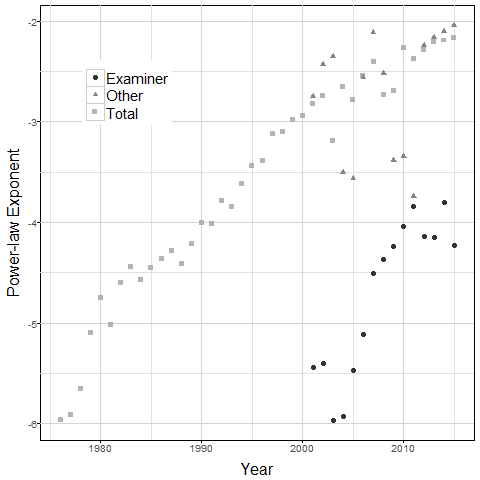
\includegraphics[width=0.7\linewidth]{Figures/paramsOverTime_pl}
  \caption[Variation of Power-Law exponent over time]{Variation in the exponent of the Power-Law fit for degree distribution from 1976:2015, where available "Examiner" and "Other" sub-graphs are also computed}
\label{fig:paramsOverTime_pl}
\end{figure}

\begin{figure}
\centering
\begin{subfigure}{.5\textwidth}
  \centering
  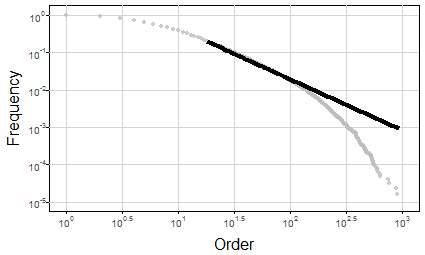
\includegraphics[width=0.9\linewidth]{Figures/plFit2003}
 \caption[]{\small Power-Law fit for "Other" sub-graph in 2003}
\label{fig:plFit2003}
\end{subfigure}%
\begin{subfigure}{.5\textwidth}
  \centering
  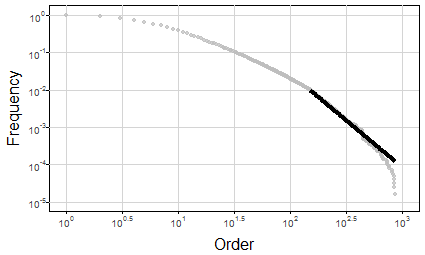
\includegraphics[width=0.9\linewidth]{Figures/plFit2004}
  \caption[]{\small Power-Law fit for "Other" sub-graph in 2004}
\label{fig:plFit2004}
\end{subfigure}
\caption[Power-law fitting to different parts of the curve for the "Other" sub-graph]{}
\label{fig:plFits}
\end{figure}

\begin{figure}
\centering
\begin{subfigure}{.7\textwidth}
  \centering
  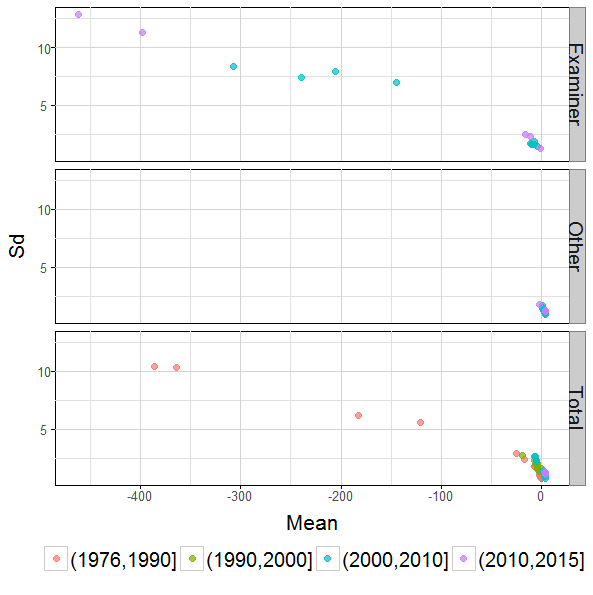
\includegraphics[width=0.9\linewidth]{Figures/logNormalParams}
 \caption[]{\small Overview}
\label{fig:logNormalParams}
\end{subfigure}%

\begin{subfigure}{.7\textwidth}
  \centering
  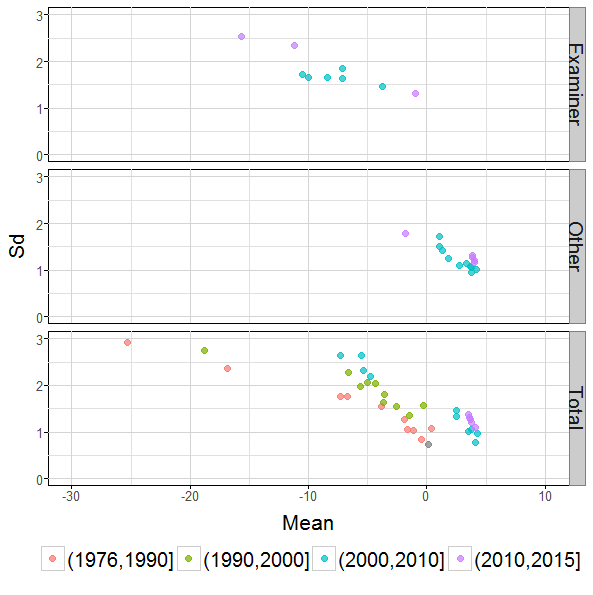
\includegraphics[width=0.9\linewidth]{Figures/logNormalParams_zoomed}
  \caption[]{\small Zoomed in on cluster}
\label{fig:logNormalParams_zoomed}
\end{subfigure}
\caption[Variation of Log-normal parameters over time]{Variation in the mean and standard deviation of log-normal fits each year 1976 to 2015 for cited by "Examiner", cited by "Other" and combined. Colour representing the decade}
\label{fig:logNormalParamPlots}
\end{figure} 
%\include{Chapters/Chapter5}
% Chapter Template

\chapter{Conclusion} % Main chapter title
	
\label{ChapterX} % Change X to a consecutive number; for referencing this chapter elsewhere, use \ref{ChapterX}

%----------------------------------------------------------------------------------------
%	SECTION 1
%----------------------------------------------------------------------------------------

\section{Review}

While we have not tested for distributions such exponential cut-off to power law distributions or extended power laws, we have analytically shown the log-normal is the most likely fit to the overall degree-distribution of the current network. The chance of a power-law fit is sufficiently unlikely that it can be discounted as a hypothesis through bootstrapping and log-likelihood comparisons. 

The network has evolved to this point at the beginning of the data-set comparison techniques couldn't distinguish between power-law and log-normal distributions but were in favour of power-law while over time the distribution is became less similar to a power-law and more similar to a log-normal.

We coloured the network into two classes from 2001 to 2015 depending on the role of the individual making the citation, the Examiner network and the Other network. We found that these are fairly disparate networks with small negative correlations between the two and different functional forms (although small positive correlations at extreme order values). The Other citations dominate in number so their structure is similar to that found in the aggregate over these years but the Examiner network seems to emulate the aggregate network in the years before these classes could be distinguished (1976 to 2000), with log-normal parameters fits similar to these times and Power-law/log-normal P values calculated yielding similar results, i.e. that neither power-law and log-normal can be discounted but the power-law is more likely (P = 0.637). Finally the average number of citations changing with time showing significant growth in the Other network further drowning out the Examiner network but supporting a hypothesis that in the past the Other network smaller relative to the Examiner and that this change in how applicants are interacting with patents is the cause of a lot of the changes in the patent network over the last decade. 

\section{Further Research}

As mentioned in the introduction showing a log-normal or power-law form is not sufficient to identify preferential attachment or other such mechanisms. Considering the contradicting research in the USPTO data-set research identifying the presence and nature of any preferential attachment mechanisms is important future research. 

One of the main research questions of this project was to identify the structural changes to the patent network over time and relate that to claims of an information revolution or economic identifiers. While we have shown there are major structural changes and that they are linked to the change in interaction of the applicant of a patent. This hasn't been linked to external factors. Further research could seek to achieve this in a number of ways, correlating changes to the patent system with econometric information answering questions like how is innovation affected by recession. More importantly would be through studying the how the technology sectors vary,  identified large structural differences between technology sectors, relating this research with temporal changes can give a much better idea of how innovation shifts between different technological areas \cite{gress2010properties}. 

The nature of the different classes of citation form different types of relationship between the same nodes. This can be represented as an unweighted multi-layer network. Representing the network in this manner can allow for techniques which study the whole network in a way which doesn't ignore the different nature of relationship between an Examiner citation and a Applicant citation \cite{hardtoSpell}. 

Finally a more directly practical direction for further research can focus on the prediction of success, and evaluation of value to the network of different patents. While research has been done on these topics adding the additional features and information from the Examiner network may improve the accuracy of these models. Additionally the extra features may prove useful in other ways such as clustering algorithms and anomaly detection in order to identify patent trolls.  


%----------------------------------------------------------------------------------------
%	THESIS CONTENT - APPENDICES
%----------------------------------------------------------------------------------------

\appendix % Cue to tell LaTeX that the following "chapters" are Appendices

% Include the appendices of the thesis as separate files from the Appendices folder
% Uncomment the lines as you write the Appendices

% Appendix A

\chapter{Document Parsing Function} % Main appendix title

\label{AppendixA} % For referencing this appendix elsewhere, use \ref{AppendixA}
\tiny
\begin{lstlisting}[language=R]

parse <- function(input_path, type, output_path_patent, output_path_citation) {
    # Libraries 
    require(stringr)
    require(readr)
    
    # Save environment to reference
    Env <- environment()
    
    # Create output paths if they don't exist
    dirs <- str_replace_all(c(output_path_patent, output_path_citation), "/.+.csv$", "")
    sapply(dirs, function(dir) {
        if (!dir.exists(dir)) dir.create(dir, recursive = T)
    })
    
    # Actions ##########################################################
    
    # Initialise output vecotrs for patent / citations upon reaching a new patent
    initialise_result <- function() {
        # If files don't exist write their column names
        if (!file.exists(output_path_patent)) {
            write(patent_colnames, output_path_patent, sep = ",", append = F, 
                  ncolumns = length(patent_colnames))
        }
        if (!file.exists(output_path_citation)) {
            write(citation_colnames, output_path_citation, sep = ",", append = F, 
                  ncolumns = length(citation_colnames))
        }
        patent <<- vector("character", length = length(patent_colnames))
        citations <<- NULL
        citation_current <<- vector("character", length = length(citation_colnames) - 1)
    }
    
    # Write patent / citation information to file upon finding the end of the current patent
    flush_patent <- function() {
        if (patent[1] != "") {
            # Add degree to dataframe
            nrow_citations <- nrow(citations)
            if (is.null(nrow_citations)) nrow_citations <- 0
            patent[which(patent_colnames == "Order")] <- nrow_citations
            write(patent, output_path_patent, sep = ",", 
                  append = T, ncolumns = length(patent_colnames))
            write_csv(as.data.frame(citations), output_path_citation, append = T)
        }
    }
    
    # Add current citation to citations matrix after finding the end of the current citaiton
    flush_citation <- function() {
        if (sum(citation_current != rep("", length(citation_colnames) - 1)) > 0) {
            citations <<- rbind(citations, c(patent[1], citation_current))
            citation_current <<- vector("character", length = length(citation_colnames) - 1)
        }
    }
    
    # Upon finding relevant information add to patent/citation output
    add_patent_information <- function(tag = line_tag, State = state, 
                                       vars = tag_add_patent_information) {
        if (State != "patent") return()
        ii <- match(tag, vars)
        patent[ii] <<- contents()
    }
    
    add_citation_information <- function(tag = line_tag, State = state, 
                                         vars = tag_add_citation_information) {
        if (State != "citation") return()
        ii <- match(tag, vars)
        citation_current[ii] <<- contents()
    }
    
    # State change: upon reaching different sections change state 
    state_change_patent <- function() {
        state <<- "patent"
    }
    state_change_citation <- function() {
        state <<- "citation"
    }
    state_change_none <- function() {
        state <<- "none"
    }
    
    # Function to get contents (so not evaluated every line) 
    contents <- function(line = Env$line, type = Env$type) {
        ifelse(type == "text",
               str_trim(substring(line, 5)),
               str_replace_all(line, "<.*?>", ""))
    } 
    
    # If sgml check for citation and country information hidden inside the tag
    sgml_exceptions <- function(line) {
        if (grepl("(<CITED-BY-OTHER/>)|(<CITED-BY-OTHER>)", line)) {
            citation_current[which(citation_colnames == "Cited by") - 1] <<- "cited by other"    
        } else if (grepl("(<CITED-BY-EXAMINER/>)|(<CITED-BY-EXAMINER>)", line)){
            citation_current[which(citation_colnames == "Cited by") - 1] <<- "cited by examiner"    
        }
        if (grepl("<PARTY-US>", line)) {
            citation_current[which(citation_colnames == "Country") - 1] <<- "US"
        }
        # Remove some extra tags which create duplicate matches
        line <- str_replace(line, "(</DOC>)|(<CITED-BY-OTHER/>)|(<CITED-BY-EXAMINER/>)|
                            (<PARTY-US>)|(<CITED-BY-OTHER>)|(<CITED-BY-EXAMINER>)", "")
        return(line)
    }
    
    ## initialisation ###################################################
    state <- "patent"
    # List the tags associated with each action function
    switch(type,
           text = {
               tag_initialise_result <- "PATN"
               tag_flush_patent <- "PATN"
               tag_flush_citation <- c("UREF", "FREF", "OREF", "DRWD", "PATN")
               tag_add_patent_information <- c("WKU ", "ISD ")
               tag_add_citation_information <- c( "PNO ", "ISD ")
               tag_state_change_citation <- c("UREF", "FREF")
               tag_state_change_patent <- "PATN"
               tag_state_change_none <- c("INVT","CLAS")
           },
           xml = {
               tag_initialise_result <- '<?xml version="1.0" encoding="UTF-8"?>'
               tag_flush_patent <- '</us-patent-grant>'
               tag_flush_citation <- c("</us-citation>", "</citation>")
               tag_add_patent_information <- c("<doc-number></doc-number>", "<date></date>",
                                               "<main-classification></main-classification>", 
                                               "<further-classification></further-classification>")
               tag_add_citation_information <- c("<doc-number></doc-number>", "<date></date>", 
                                                 "<category></category>", "<country></country>")
               tag_state_change_citation <- c("<us-citation>", "<citation>")
               tag_state_change_patent <- c("<publication-reference>", "<classification-national>")
               tag_state_change_none <- c("</publication-reference>", "</us-ciation>", 
                                          "</citation>", "</classification-national>")
               citation_colnames <- c("Patent", "Citation", "Date", "CitedBy", "Country")
               patent_colnames <- c("Patent", "Date", "MainClassification", "FurtherClassification", "Order")
           },
           sgml = {
               tag_initialise_result <- '<SDOBI>'
               tag_flush_patent <- "</SDOBI>"
               tag_flush_citation <- "</B561>"
               tag_add_patent_information <- c("<B110><DNUM><PDAT></PDAT></DNUM></B110>", # patent number
                                               "<B140><DATE><PDAT></PDAT></DATE></B140>", # Date
                                               "<B521><PDAT></PDAT></B521>", # Main classification,
                                               "<B522><PDAT></PDAT></B522>") # Further classification
               tag_add_citation_information <- c("<DOC><DNUM><PDAT></PDAT></DNUM>", # Patent number
                                                 "<DATE><PDAT></PDAT></DATE>", # Patent Date
                                                 "<CTRY><PDAT></PDAT></CTRY>") # Country
               tag_state_change_citation <- "<B561>"
               tag_state_change_patent <- '<SDOBI>'
               tag_state_change_none <- NULL
               citation_colnames <- c("Patent", "Citation", "Date", "CitedBy", "Country")
               patent_colnames <- c("Patent", "Date", "MainClassification", "FurtherClassification", "Order")
           })
    
    # Initialise total taglist and response index
    tag_list <- list(tag_flush_citation, tag_flush_patent, tag_state_change_patent, 
                     tag_state_change_citation, tag_state_change_none, tag_initialise_result,
                     tag_add_citation_information, tag_add_patent_information)
    tag_all <- unlist(tag_list)
    tag_index <- rep(1:length(tag_list), sapply(tag_list, length))
    # Vectorise action functions in same order as tags which call them
    action_functions <- list(flush_citation, flush_patent,  state_change_patent, 
                             state_change_citation, state_change_none, initialise_result,
                             add_citation_information, add_patent_information)
    
    # Read data
    text <- read_lines(input_path)
    
    ## LOOP ############################################################
    pb <- txtProgressBar(min = 0, max = length(text), initial = 0, style = 3)
    initialise_result()
    for (i in seq_along(text)) {
        line <- text[i]
        if (i %% 1000 == 0) setTxtProgressBar(pb, i)
        
        # Turn current line into a tag (acts differently for text / sgml)
        line_tag <- ifelse(type == "text", 
                           substring(line, 1, 4), 
                           str_replace_all(line, ">.*?<", "><")
                           )
        
        if (type == "sgml") line_tag <- sgml_exceptions(line_tag)
    
        # Check if it matches any in the list 
        matches <- tag_index[tag_all %in% line_tag]
        
        # If match occurs invoke the appropriate action function
        if (length(matches) > 0) {
            lapply(matches, function(x) action_functions[[x]]())
        }
    }
    if (type == "text") flush_patent() #Because text doesn't have close tags
    close(pb)
}

\end{lstlisting}


% Appendix Template

\chapter{Example Raw Data Patent: Text format} % Main appendix title

\label{AppendixB} % Change X to a consecutive letter; for referencing this appendix elsewhere, use \ref{AppendixX}

\tiny 
\begin{lstlisting}

PATN
WKU  RE0286710
SRC  5
APN  500649\&
APT  2
PBL  E
ART  315
APD  19740826
TTL  Hydrophone damper assembly
ISD  19760106
NCL  18
ECL  13
EXA  Basinger; Sherman D.
EXP  Blix; Trygve M.
NDR  2
NFG  10
INVT
NAM  Widenhofer; James W.
CTY  Jackson
STA  MI
ASSG
NAM  Sparton Corporation
CTY  Jackson
STA  MI
COD  02
REIS
COD  50
APN  151269
APD  19710609
PNO  03701175
ISD  19721031
CLAS
OCL    9  8R
XCL  340  2
XCL  340  3T
XCL  340  7R
XCL  340  8R
EDF  2
ICL  B63B 2152
ICL  B63B 5102
FSC    9
FSS  8 R
FSC  340
FSS  2;3 T;8 S;8 R;7
FSC  114
FSS  206 R
UREF
PNO  2790186
ISD  19570400
NAM  Carapellotti
OCL    9  8R
UREF
PNO  3329015
ISD  19670700
NAM  Bakeke et al.
OCL  340  2
UREF
PNO  3377615
ISD  19680400
NAM  Lutes
OCL  340  2
UREF
PNO  3543228
ISD  19701100
NAM  Farmer
OCL  340  2
UREF
PNO  3543228
ISD  19701100
NAM  Farmer et al.
OCL    9  8R
UREF
PNO  3711821
ISD  19730100
NAM  Dale et al.
OCL    9  8R
UREF
PNO  3720909
ISD  19730300
NAM  Sikora
OCL  340  2
UREF
PNO  3803540
ISD  19740400
NAM  Mar et al.
OCL  340  2
LREP
FRM  Beaman \& Beaman
ABST
PAL  A damper for use in submerged hydrophone suspension systems including an
      elongated mass cylinder defined by a tube of flexible synthetic plastic
      film utilizing a check valve located at each end permitting water to enter
      the tube and preventing egress. Additionally, each tube end is provided
      with a disk transversely disposed to the tube length and of a diameter
      substantially greater than that of the tube to provide drag and
      hydrodynamic mass damping. The tube and disk are of a configuration to
      eliminate vortex shedding and the entire damper assembly is capable of
      being folded and packed within a concise configuration prior to
      deployment.
      
\end{lstlisting}
% Appendix Template

\chapter{Example Raw Data Patent: Sgml format} % Main appendix title

\label{AppendixC} % Change X to a consecutive letter; for referencing this appendix elsewhere, use \ref{AppendixX}

\tiny
\begin{lstlisting}

<?xml version="1.0" encoding="UTF-8"?>
<!DOCTYPE PATDOC SYSTEM "ST32-US-Grant-025xml.dtd" [
<!ENTITY USD0468513-20030114-D00000.TIF SYSTEM "USD0468513-20030114-D00000.TIF" NDATA TIF>
<!ENTITY USD0468513-20030114-D00001.TIF SYSTEM "USD0468513-20030114-D00001.TIF" NDATA TIF>
<!ENTITY USD0468513-20030114-D00002.TIF SYSTEM "USD0468513-20030114-D00002.TIF" NDATA TIF>
<!ENTITY USD0468513-20030114-D00003.TIF SYSTEM "USD0468513-20030114-D00003.TIF" NDATA TIF>
]>
<PATDOC DTD="2.5" STATUS="Build 20020918">
<SDOBI>
<B100>
<B110><DNUM><PDAT>D0468513</PDAT></DNUM></B110>
<B130><PDAT>S1</PDAT></B130>
<B140><DATE><PDAT>20030114</PDAT></DATE></B140>
<B190><PDAT>US</PDAT></B190>
</B100>
<B200>
<B210><DNUM><PDAT>29152580</PDAT></DNUM></B210>
<B211US><PDAT>29</PDAT></B211US>
<B220><DATE><PDAT>20011227</PDAT></DATE></B220>
</B200>
<B300>
<B310><DNUM><PDAT>1999-2430 CA</PDAT></DNUM></B310>
<B320><DATE><PDAT>19991006</PDAT></DATE></B320>
<B330><CTRY><PDAT>CA</PDAT></CTRY></B330>
</B300>
<B400>
<B472>
<B474><PDAT>14</PDAT></B474>
</B472>
</B400>
<B500>
<B510>
<B511><PDAT>0101</PDAT></B511>
<B516><PDAT>7</PDAT></B516>
</B510>
<B520>
<B521><PDAT>D 1104</PDAT></B521>
</B520>
<B540><STEXT><PDAT>Lollipop</PDAT></STEXT></B540>
<B560>
<B561>
<PCIT>
<DOC><DNUM><PDAT>1257779</PDAT></DNUM>
<DATE><PDAT>19180200</PDAT></DATE>
<KIND><PDAT>A</PDAT></KIND>
</DOC>
<PARTY-US>
<NAM><SNM><STEXT><PDAT>Anderson</PDAT></STEXT></SNM></NAM>
</PARTY-US>
<PNC><PDAT>273146</PDAT></PNC></PCIT><CITED-BY-EXAMINER/>
</B561>
<B561>
<PCIT>
<DOC><DNUM><PDAT>D58042</PDAT></DNUM>
<DATE><PDAT>19210500</PDAT></DATE>
<KIND><PDAT>S</PDAT></KIND>
</DOC>
<PARTY-US>
<NAM><SNM><STEXT><PDAT>Paine</PDAT></STEXT></SNM></NAM>
</PARTY-US>
<PNC><PDAT>D 1106</PDAT></PNC></PCIT><CITED-BY-EXAMINER/>
</B561>
<B561>
<PCIT>
<DOC><DNUM><PDAT>1539015</PDAT></DNUM>
<DATE><PDAT>19250500</PDAT></DATE>
<KIND><PDAT>A</PDAT></KIND>
</DOC>
<PARTY-US>
<NAM><SNM><STEXT><PDAT>Michell</PDAT></STEXT></SNM></NAM>
</PARTY-US>
<PNC><PDAT>273146</PDAT></PNC></PCIT><CITED-BY-EXAMINER/>
</B561>
<B561>
<PCIT>
<DOC><DNUM><PDAT>1786606</PDAT></DNUM>
<DATE><PDAT>19301200</PDAT></DATE>
<KIND><PDAT>A</PDAT></KIND>
</DOC>
<PARTY-US>
<NAM><SNM><STEXT><PDAT>Gordon</PDAT></STEXT></SNM></NAM>
</PARTY-US>
<PNC><PDAT>426 91 X</PDAT></PNC></PCIT><CITED-BY-EXAMINER/>
</B561>
<B561>
<PCIT>
<DOC><DNUM><PDAT>2036706</PDAT></DNUM>
<DATE><PDAT>19360400</PDAT></DATE>
<KIND><PDAT>A</PDAT></KIND>
</DOC>
<PARTY-US>
<NAM><SNM><STEXT><PDAT>Law</PDAT></STEXT></SNM></NAM>
</PARTY-US>
<PNC><PDAT>426 85</PDAT></PNC></PCIT><CITED-BY-EXAMINER/>
</B561>
<B561>
<PCIT>
<DOC><DNUM><PDAT>2191352</PDAT></DNUM>
<DATE><PDAT>19400200</PDAT></DATE>
<KIND><PDAT>A</PDAT></KIND>
</DOC>
<PARTY-US>
<NAM><SNM><STEXT><PDAT>Oprean</PDAT></STEXT></SNM></NAM>
</PARTY-US>
<PNC><PDAT>426101</PDAT></PNC></PCIT><CITED-BY-EXAMINER/>
</B561>
<B561>
<PCIT>
<DOC><DNUM><PDAT>2589823</PDAT></DNUM>
<DATE><PDAT>19520300</PDAT></DATE>
<KIND><PDAT>A</PDAT></KIND>
</DOC>
<PARTY-US>
<NAM><SNM><STEXT><PDAT>Krens</PDAT></STEXT></SNM></NAM>
</PARTY-US>
<PNC><PDAT>426421</PDAT></PNC></PCIT><CITED-BY-EXAMINER/>
</B561>
<B561>
<PCIT>
<DOC><DNUM><PDAT>3062662</PDAT></DNUM>
<DATE><PDAT>19621100</PDAT></DATE>
<KIND><PDAT>A</PDAT></KIND>
</DOC>
<PARTY-US>
<NAM><SNM><STEXT><PDAT>McDonald</PDAT></STEXT></SNM></NAM>
</PARTY-US>
<PNC><PDAT>426 91 X</PDAT></PNC></PCIT><CITED-BY-EXAMINER/>
</B561>
<B561>
<PCIT>
<DOC><DNUM><PDAT>3400932</PDAT></DNUM>
<DATE><PDAT>19680900</PDAT></DATE>
<KIND><PDAT>A</PDAT></KIND>
</DOC>
<PARTY-US>
<NAM><SNM><STEXT><PDAT>Conrad</PDAT></STEXT></SNM></NAM>
</PARTY-US>
<PNC><PDAT>273146</PDAT></PNC></PCIT><CITED-BY-EXAMINER/>
</B561>
<B561>
<PCIT>
<DOC><DNUM><PDAT>3459296</PDAT></DNUM>
<DATE><PDAT>19690800</PDAT></DATE>
<KIND><PDAT>A</PDAT></KIND>
</DOC>
<PARTY-US>
<NAM><SNM><STEXT><PDAT>Berg</PDAT></STEXT></SNM></NAM>
</PARTY-US>
<PNC><PDAT>426134 X</PDAT></PNC></PCIT><CITED-BY-EXAMINER/>
</B561>
</B560>
<B570>
<B577><PDAT>1</PDAT></B577>
<B578US><PDAT>1</PDAT></B578US>
</B570>
<B580>
<B583US><PDAT>D 1100-129</PDAT></B583US>
<B582><PDAT>D 1199</PDAT></B582>
<B582><PDAT>426 85</PDAT></B582>
<B582><PDAT>426 90</PDAT></B582>
<B582><PDAT>426 91</PDAT></B582>
<B583US><PDAT>426100-104</PDAT></B583US>
<B583US><PDAT>426132-134</PDAT></B583US>
<B582><PDAT>426249</PDAT></B582>
<B582><PDAT>426801</PDAT></B582>
<B582><PDAT>426421</PDAT></B582>
<B582><PDAT>426660</PDAT></B582>
<B582><PDAT>273146</PDAT></B582>
<B582><PDAT>273260</PDAT></B582>
<B582><PDAT> 21372</PDAT></B582>
<B582><PDAT> 21373</PDAT></B582>
<B582><PDAT> 21347</PDAT></B582>
<B582><PDAT> 21499</PDAT></B582>
</B580>
<B590><B595><PDAT>3</PDAT></B595><B596><PDAT>9</PDAT></B596><B597US/>
</B590>
</B500>
<B600>
<B630><B632><PARENT-US><CDOC><DOC><DNUM><PDAT>29/152580</PDAT></DNUM></DOC></CDOC><PDOC><DOC><DNUM><PDAT>29/121438</PDAT></DNUM><DATE><PDAT>20000406</PDAT></DATE><CTRY><PDAT>US</PDAT></CTRY><KIND><PDAT>00</PDAT></KIND></DOC></PDOC><PSTA><PDAT>03</PDAT></PSTA></PARENT-US></B632></B630>
</B600>
<B700>
<B720>
<B721>
<PARTY-US>
<NAM><FNM><PDAT>Lisa Jane</PDAT></FNM><SNM><STEXT><PDAT>Wolfe</PDAT></STEXT></SNM></NAM>
<ADR>
<STR><PDAT>8700 No. 52nd St.</PDAT></STR>
<CITY><PDAT>Paradise Valley</PDAT></CITY>
<STATE><PDAT>AZ</PDAT></STATE>
<PCODE><PDAT>85253</PDAT></PCODE>
</ADR>
</PARTY-US>
</B721>
<B721>
<PARTY-US>
<NAM><FNM><PDAT>Jane Margaret</PDAT></FNM><SNM><STEXT><PDAT>Bachynski</PDAT></STEXT></SNM></NAM>
<ADR>
<STR><PDAT>&num;6-55 Whitemarl Dr.</PDAT></STR>
<CITY><PDAT>Rockcliffe Park Ontario</PDAT></CITY>
<CTRY><PDAT>CA</PDAT></CTRY>
<PCODE><PDAT>K1L 8J9 </PDAT></PCODE>
</ADR>
</PARTY-US>
</B721>
</B720>
<B740>
<B741>
<PARTY-US>
<NAM><ONM><STEXT><PDAT>Fulbright &amp; Jaworski, LLP</PDAT></STEXT></ONM></NAM>
</PARTY-US>
</B741>
</B740>
<B745>
<B746>
<PARTY-US>
<NAM><FNM><PDAT>Alan P.</PDAT></FNM><SNM><STEXT><PDAT>Douglas</PDAT></STEXT></SNM></NAM>
</PARTY-US>
</B746>
<B747>
<PARTY-US>
<NAM><FNM><PDAT>Linda</PDAT></FNM><SNM><STEXT><PDAT>Brooks</PDAT></STEXT></SNM></NAM>
</PARTY-US>
</B747>
<B748US><PDAT>2911</PDAT></B748US>
</B745>
</B700>
</SDOBI>
<SDODE>
</SDODE>
<SDOCL>
<CL>
<CLM ID="CLM-00001">
<PARA ID="P-00010" LVL="7"><PTEXT><PDAT>The ornamental design for a lollipop, as shown and described.</PDAT></PTEXT></PARA>
</CLM>
</CL>
</SDOCL>
</PATDOC>

\end{lstlisting}
% Appendix Template

\chapter{Example Raw Data Patent: XML format} % Main appendix title

\label{AppendixD} % Change X to a consecutive letter; for referencing this appendix elsewhere, use \ref{AppendixX}

\tiny 

\begin{lstlisting}
<?xml version="1.0" encoding="UTF-8"?>
<!DOCTYPE us-patent-grant SYSTEM "us-patent-grant-v42-2006-08-23.dtd" [ ]>
<us-patent-grant lang="EN" dtd-version="v4.2 2006-08-23" file="US07646781-20100112.XML" status="PRODUCTION" id="us-patent-grant" country="US" date-produced="20091229" date-publ="20100112">
<us-bibliographic-data-grant>
<publication-reference>
<document-id>
<country>US</country>
<doc-number>07646781</doc-number>
<kind>B2</kind>
<date>20100112</date>
</document-id>
</publication-reference>
<application-reference appl-type="utility">
<document-id>
<country>US</country>
<doc-number>11753703</doc-number>
<date>20070525</date>
</document-id>
</application-reference>
<us-application-series-code>11</us-application-series-code>
<us-term-of-grant>
<us-term-extension>402</us-term-extension>
</us-term-of-grant>
<classifications-ipcr>
<classification-ipcr>
<ipc-version-indicator><date>20060101</date></ipc-version-indicator>
<classification-level>A</classification-level>
<section>H</section>
<class>04</class>
<subclass>L</subclass>
<main-group>12</main-group>
<subgroup>56</subgroup>
<symbol-position>F</symbol-position>
<classification-value>I</classification-value>
<action-date><date>20100112</date></action-date>
<generating-office><country>US</country></generating-office>
<classification-status>B</classification-status>
<classification-data-source>H</classification-data-source>
</classification-ipcr>
</classifications-ipcr>
<classification-national>
<country>US</country>
<main-classification>370412</main-classification>
<further-classification>370235</further-classification>
</classification-national>
<invention-title id="d0e53">Methods, systems, and computer program products for selectively discarding packets</invention-title>
<references-cited>
<citation>
<patcit num="00001">
<document-id>
<country>US</country>
<doc-number>2006/0072576</doc-number>
<kind>A1</kind>
<name>Miao et al.</name>
<date>20060400</date>
</document-id>
</patcit>
<category>cited by examiner</category>
<classification-national><country>US</country><main-classification>370394</main-classification></classification-national>
</citation>
<citation>
<patcit num="00002">
<document-id>
<country>US</country>
<doc-number>2006/0291384</doc-number>
<kind>A1</kind>
<name>Harris et al.</name>
<date>20061200</date>
</document-id>
</patcit>
<category>cited by examiner</category>
<classification-national><country>US</country><main-classification>370229</main-classification></classification-national>
</citation>
<citation>
<patcit num="00003">
<document-id>
<country>US</country>
<doc-number>2007/0201365</doc-number>
<kind>A1</kind>
<name>Skoog et al.</name>
<date>20070800</date>
</document-id>
</patcit>
<category>cited by examiner</category>
<classification-national><country>US</country><main-classification>3702301</main-classification></classification-national>
</citation>
<citation>
<patcit num="00004">
<document-id>
<country>US</country>
<doc-number>2009/0129313</doc-number>
<kind>A1</kind>
<name>Tamura et al.</name>
<date>20090500</date>
</document-id>
</patcit>
<category>cited by examiner</category>
<classification-national><country>US</country><main-classification>370328</main-classification></classification-national>
</citation>
<citation>
<nplcit num="00005">
<othercit>Web page published by &#x201c;vonage.nmhoy.net/qos.html&#x201d;; http;//web.archive.org/web/20060314042029/http://vonage.nmhoy.net/qos.html; retrieved on May 8, 2007, pp. 1-5.</othercit>
</nplcit>
<category>cited by other</category>
</citation>
</references-cited>
<number-of-claims>23</number-of-claims>
<us-exemplary-claim>1</us-exemplary-claim>
<us-field-of-classification-search>
<classification-national>
<country>US</country>
<main-classification>370234</main-classification>
</classification-national>
<classification-national>
<country>US</country>
<main-classification>370229</main-classification>
</classification-national>
<classification-national>
<country>US</country>
<main-classification>370230</main-classification>
</classification-national>
<classification-national>
<country>US</country>
<main-classification>370232</main-classification>
</classification-national>
<classification-national>
<country>US</country>
<main-classification>370235</main-classification>
</classification-national>
<classification-national>
<country>US</country>
<main-classification>3702351</main-classification>
</classification-national>
<classification-national>
<country>US</country>
<main-classification>370352</main-classification>
</classification-national>
<classification-national>
<country>US</country>
<main-classification>370412</main-classification>
</classification-national>
<classification-national>
<country>US</country>
<main-classification>370428</main-classification>
</classification-national>
<classification-national>
<country>US</country>
<main-classification>370429</main-classification>
</classification-national>
<classification-national>
<country>US</country>
<main-classification>37039521</main-classification>
</classification-national>
<classification-national>
<country>US</country>
<main-classification>3703954</main-classification>
</classification-national>
<classification-national>
<country>US</country>
<main-classification>37039541</main-classification>
</classification-national>
<classification-national>
<country>US</country>
<main-classification>37039542</main-classification>
</classification-national>
<classification-national>
<country>US</country>
<main-classification>37039552</main-classification>
</classification-national>
<classification-national>
<country>US</country>
<main-classification>370470</main-classification>
</classification-national>
</us-field-of-classification-search>
<figures>
<number-of-drawing-sheets>5</number-of-drawing-sheets>
<number-of-figures>5</number-of-figures>
</figures>
<us-related-documents>
<related-publication>
<document-id>
<country>US</country>
<doc-number>20080291935</doc-number>
<kind>A1</kind>
<date>20081127</date>
</document-id>
</related-publication>
</us-related-documents>
<parties>
<applicants>
<applicant sequence="001" app-type="applicant-inventor" designation="us-only">
<addressbook>
<last-name>Campion</last-name>
<first-name>Nicholas F.</first-name>
<address>
<city>Rochester</city>
<state>MN</state>
<country>US</country>
</address>
</addressbook>
<nationality>
<country>omitted</country>
</nationality>
<residence>
<country>US</country>
</residence>
</applicant>
<applicant sequence="002" app-type="applicant-inventor" designation="us-only">
<addressbook>
<last-name>Cramer</last-name>
<first-name>Keith D.</first-name>
<address>
<city>Pine Island</city>
<state>MN</state>
<country>US</country>
</address>
</addressbook>
<nationality>
<country>omitted</country>
</nationality>
<residence>
<country>US</country>
</residence>
</applicant>
<applicant sequence="003" app-type="applicant-inventor" designation="us-only">
<addressbook>
<last-name>Morrison</last-name>
<first-name>Donald A.</first-name>
<address>
<city>Rochester</city>
<state>MN</state>
<country>US</country>
</address>
</addressbook>
<nationality>
<country>omitted</country>
</nationality>
<residence>
<country>US</country>
</residence>
</applicant>
<applicant sequence="004" app-type="applicant-inventor" designation="us-only">
<addressbook>
<last-name>Strauss</last-name>
<first-name>Daniel J.</first-name>
<address>
<city>Rochester</city>
<state>MN</state>
<country>US</country>
</address>
</addressbook>
<nationality>
<country>omitted</country>
</nationality>
<residence>
<country>US</country>
</residence>
</applicant>
</applicants>
<agents>
<agent sequence="01" rep-type="attorney">
<addressbook>
<orgname>Cantor Colburn, LLP</orgname>
<address>
<country>unknown</country>
</address>
</addressbook>
</agent>
</agents>
</parties>
<assignees>
<assignee>
<addressbook>
<orgname>International Business Machines Corporation</orgname>
<role>02</role>
<address>
<city>Armonk</city>
<state>NY</state>
<country>US</country>
</address>
</addressbook>
</assignee>
</assignees>
<examiners>
<primary-examiner>
<last-name>Nguyen</last-name>
<first-name>Brian D</first-name>
<department>2416</department>
</primary-examiner>
</examiners>
</us-bibliographic-data-grant>
<abstract id="abstract">
<p id="p-0001" num="0000">A method, system, and computer program product are provided for selectively discarding packets in a network device. The method includes receiving an upstream bandwidth saturation indicator for a queue in the network device, and identifying one or more codecs employed in packets in the queue when the upstream bandwidth saturation indicator indicates saturation. The method further includes determining a packet discarding policy based on the one or more codecs, and discarding packets in accordance with the packet discarding policy.</p>
</abstract>
</us-patent-grant>
\end{lstlisting}

%----------------------------------------------------------------------------------------
%	BIBLIOGRAPHY
%----------------------------------------------------------------------------------------

\printbibliography[heading=bibintoc]

%----------------------------------------------------------------------------------------

\end{document}  
